\chapter{Vento a 10 metros}\label{cap:resultados_wind10}

Nos ciclones extratropicais (ETC), o vento em superfície favorece a formação de ondas anômalas \citep{gramcianinov2023impact}.
Esse vento responde a processos de diferentes escalas, como o fluxo sinótico, os jatos de mesoescala, as correntes descendentes e a seclusão quente (Seção~\ref{subsec:tb_modelos}).
Consequentemente, sua intensidade e distribuição espacial diferem entre ciclones, desde sistemas fracos dominados pelo fluxo de fundo até sistemas intensos que concentram os ventos mais fortes em setores específicos.

Este capítulo descreve a distribuição espacial do vento a 10 metros durante o ciclo de vida dos ETC formados nas três regiões de estudo (SBR, LPB e ARG), com três objetivos: (i)~quantificar a variação da magnitude do vento segundo a intensidade do ciclone e sua região de gênese, (ii)~identificar a localização preferencial dos máximos de vento em relação ao centro do ciclone, e (iii)~identificar os padrões dominantes de variabilidade espacial do vento e sua evolução entre fases.
A Seção~\ref{sec:pdf_wind10} compara as distribuições de magnitude (PDF) da População Global (PG) e do subconjunto de ciclones intensos (p90; Seção~\ref{subsec:subconjuntos_intensidad}).
As Seções~\ref{sec:kde_espacial_global} e~\ref{sec:kde_espacial_p90} analisam a localização dos máximos mediante sua densidade espacial (PDFe; Seção~\ref{subsec:kde_localizacion}), e as Seções~\ref{sec:var_exp_wind10}--\ref{subsec:res_dinamica_pc1} aplicam funções ortogonais empíricas (EOF; Seção~\ref{subsec:eof_univariado}) para identificar os padrões dominantes.
O Capítulo~\ref{cap:resultados_tp} aplica a mesma análise à precipitação, e o Capítulo~\ref{chap:meof} avalia se os máximos de ambas as variáveis coincidem no espaço (Seção~\ref{sec:tb_compound_def}).

% --- SEÇÃO PRINCIPAL: PDF DE VENTO A 10 METROS,
\section{Distribuição de magnitudes (PDF)}\label{sec:pdf_wind10}

A Figura~\ref{fig:pdf_wind10} apresenta as funções de densidade de probabilidade (PDF) dos máximos de vento a 10~m, extraídos do domínio centrado no ciclone (Seção~\ref{subsec:extraccion_pdf}), para as duas populações de estudo (Seção~\ref{sec:poblaciones_estudio}).
Os painéis se organizam por região de ciclogênese (SBR, LPB e ARG; Seção~\ref{sec:tb_regiones}) e por fase do ciclo de vida (Ic, It, M e D; Seção~\ref{subsec:tb_fases}).

Na fase incipiente (Ic; painéis a, b e~c), ambas as populações apresentam distribuições unimodais que se superpõem em grande parte, com picos entre 11 e 15~m\,s$^{-1}$.
Na intensificação (It; painéis d, e e~f) e na maturidade (M; painéis g, h e~i), a curva de p90 se desloca para valores maiores e alcança na maturidade um pico entre 23 e 25~m\,s$^{-1}$, com caudas de até 30~m\,s$^{-1}$.
Nessa fase, a População Global apresenta seu máximo entre 16 e 19~m\,s$^{-1}$ e uma distribuição mais larga.
Entre regiões, os picos de p90 na maturidade são mais altos em LPB (h) e ARG (i) (${\sim}0.19$) do que em SBR (g) (${\sim}0.17$), cuja distribuição é mais larga por um ombro em direção a 22--23~m\,s$^{-1}$, enquanto ARG estende sua cauda até os 30~m\,s$^{-1}$.
No decaimento (D; painéis j, k e~l), as curvas de p90 se deslocam para magnitudes menores e se alargam, embora se mantenham acima da População Global, com maior superposição em ARG.

\begin{figure}[htbp]
\centering
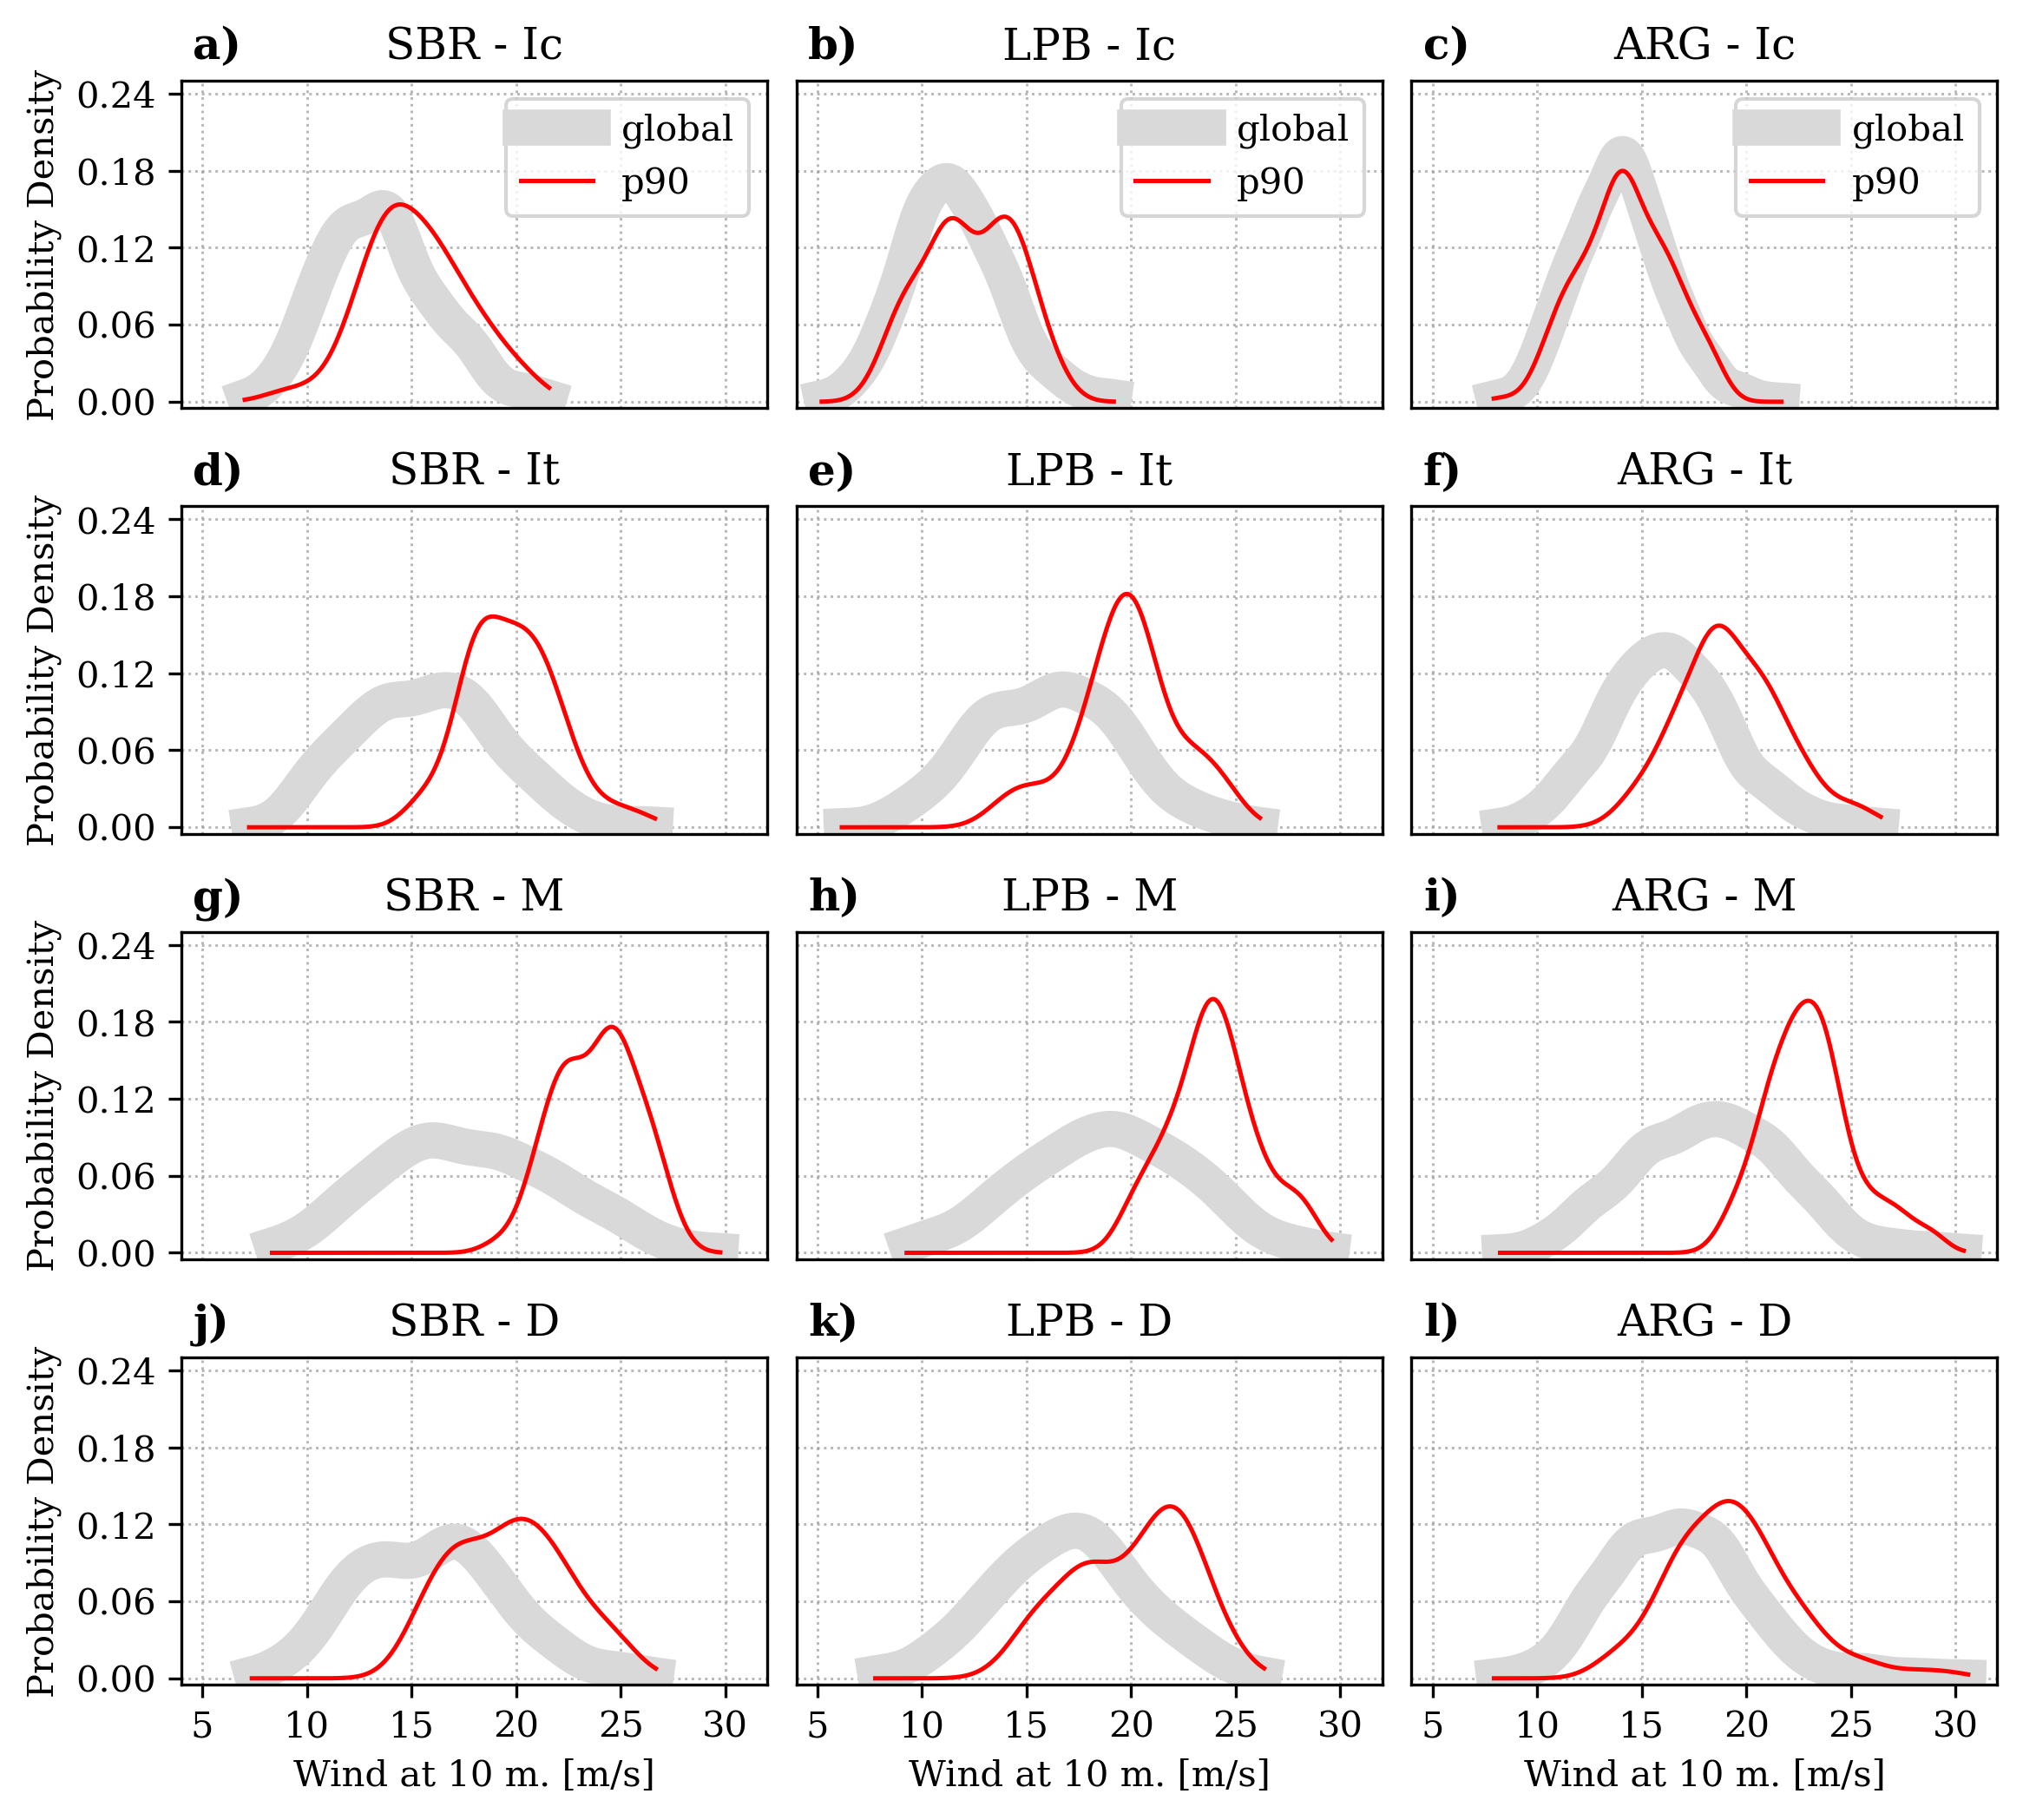
\includegraphics[width=\textwidth]{images/w10/PDF_wind10_sigma025.png}
\caption[PDF de magnitudes máximas de vento a 10 metros]{Funções de densidade de probabilidade (PDF) para as magnitudes máximas de vento a 10 metros. As colunas indicam a região de ciclogênese (SBR, LPB, ARG) e as linhas a evolução ao longo das fases do ciclo de vida (Ic, It, M, D). Contrasta-se a População Global (referência, sombreado cinza) com o subconjunto p90, formado pelos 10\% de ciclones de maior intensidade em vorticidade relativa a 850~hPa (Seção~\ref{subsec:subconjuntos_intensidad}), em linha vermelha.}
\label{fig:pdf_wind10}
\end{figure}

A maior separação entre distribuições ocorre na maturidade, fase em que a maioria dos ciclones alcança seu mínimo de vorticidade a 850~hPa, tanto na População Global quanto em p90 (Tabela~\ref{tab:fase_max_intensidad}).
\citet{gramcianinov2019properties}, a partir do vento máximo a 925~hPa, associam os ciclones de SBR e LPB a ventos intensos e apontam LPB como a região com os ciclones mais intensos do Atlântico Sul, e atribuem a ciclogênese ao norte de 35\textdegree S ao forçamento de níveis baixos ligado ao transporte de umidade no verão (Seções~\ref{subsec:tb_sbr} e~\ref{subsec:tb_lpb}). Nos dados aqui analisados, a moda da População Global na maturidade é maior em LPB (19~m\,s$^{-1}$) e ARG (18.5~m\,s$^{-1}$) do que em SBR (16~m\,s$^{-1}$), enquanto os picos de p90 são semelhantes entre regiões.

Em ARG, a baroclinicidade associada à frente e a perturbação topográfica dos Andes (Seção~\ref{subsec:tb_arg}) poderiam gerar respostas do vento mais variáveis, compatíveis com a cauda mais estendida em direção a velocidades altas que apresenta sua distribuição p90 na maturidade e no decaimento.
Apesar da menor disponibilidade de umidade, \citet{gramcianinov2024early} mostram que a amplificação da onda baroclínica em níveis baixos produz em ARG, durante a etapa inicial, ciclones com pressão central mais baixa do que em SBR e LPB, consistente com o regime mais baroclínico que caracteriza essa região.

A separação entre p90 e a População Global, que aumenta à medida que os ciclones maturam, mostra que a maior intensidade em vorticidade a 850~hPa, critério com o qual se define p90 (Seção~\ref{sec:poblaciones_estudio}), se traduz em ventos mais intensos em superfície.
Na maturidade, a moda de p90 se situa entre 23 e 25~m\,s$^{-1}$, entre 25\% (LPB e ARG) e 50\% (SBR) acima da moda da População Global (16--19~m\,s$^{-1}$), com caudas de até 30~m\,s$^{-1}$.
Esses valores são coerentes com os reportados para ciclones do Atlântico Sul \citep{padilhareinke2026characterization, gramcianinov2020analysis}.
\citet{padilhareinke2026characterization} documentam para o conjunto do Atlântico Sul-Ocidental um limiar p90 de 23.4~m\,s$^{-1}$ (84.4~km\,h$^{-1}$) e extremos de até 31.4~m\,s$^{-1}$ (113.2~km\,h$^{-1}$).
Esse limiar é semelhante ao máximo médio (${\sim}$25~m\,s$^{-1}$) do composto dos 100 ciclones mais intensos do Atlântico Norte no momento de máxima vorticidade \citep{gentile2025response}, embora se trate de outra população e outra bacia.
\citet{gramcianinov2020analysis} reportam para o inverno austral (JJA) no ERA5 velocidades máximas médias de 21.2\,$\pm$\,4.8~m\,s$^{-1}$ (percentil~90: 27.3~m\,s$^{-1}$; percentil~95: 29.3~m\,s$^{-1}$).\footnote{Na reanálise CFSR/CFSv2, os valores são ligeiramente superiores, 23.4\,$\pm$\,4.8~m\,s$^{-1}$ (percentil~90: 30.2~m\,s$^{-1}$; percentil~95: 32.1~m\,s$^{-1}$) \citep{gramcianinov2020analysis}.}
\citet{gramcianinov2023impact} destacam que as ondas extremas geradas pelos ventos desses ciclones têm um impacto considerável nas atividades costeiras e marítimas.

% --- SEÇÃO PRINCIPAL: KDE ESPACIAL DE VENTO A 10 METROS,

\section{Distribuição espacial de máximos (PDFe)}\label{sec:pdfe_wind10}
\subsection{População Global}\label{sec:kde_espacial_global}

\begin{figure}[htbp]
\centering
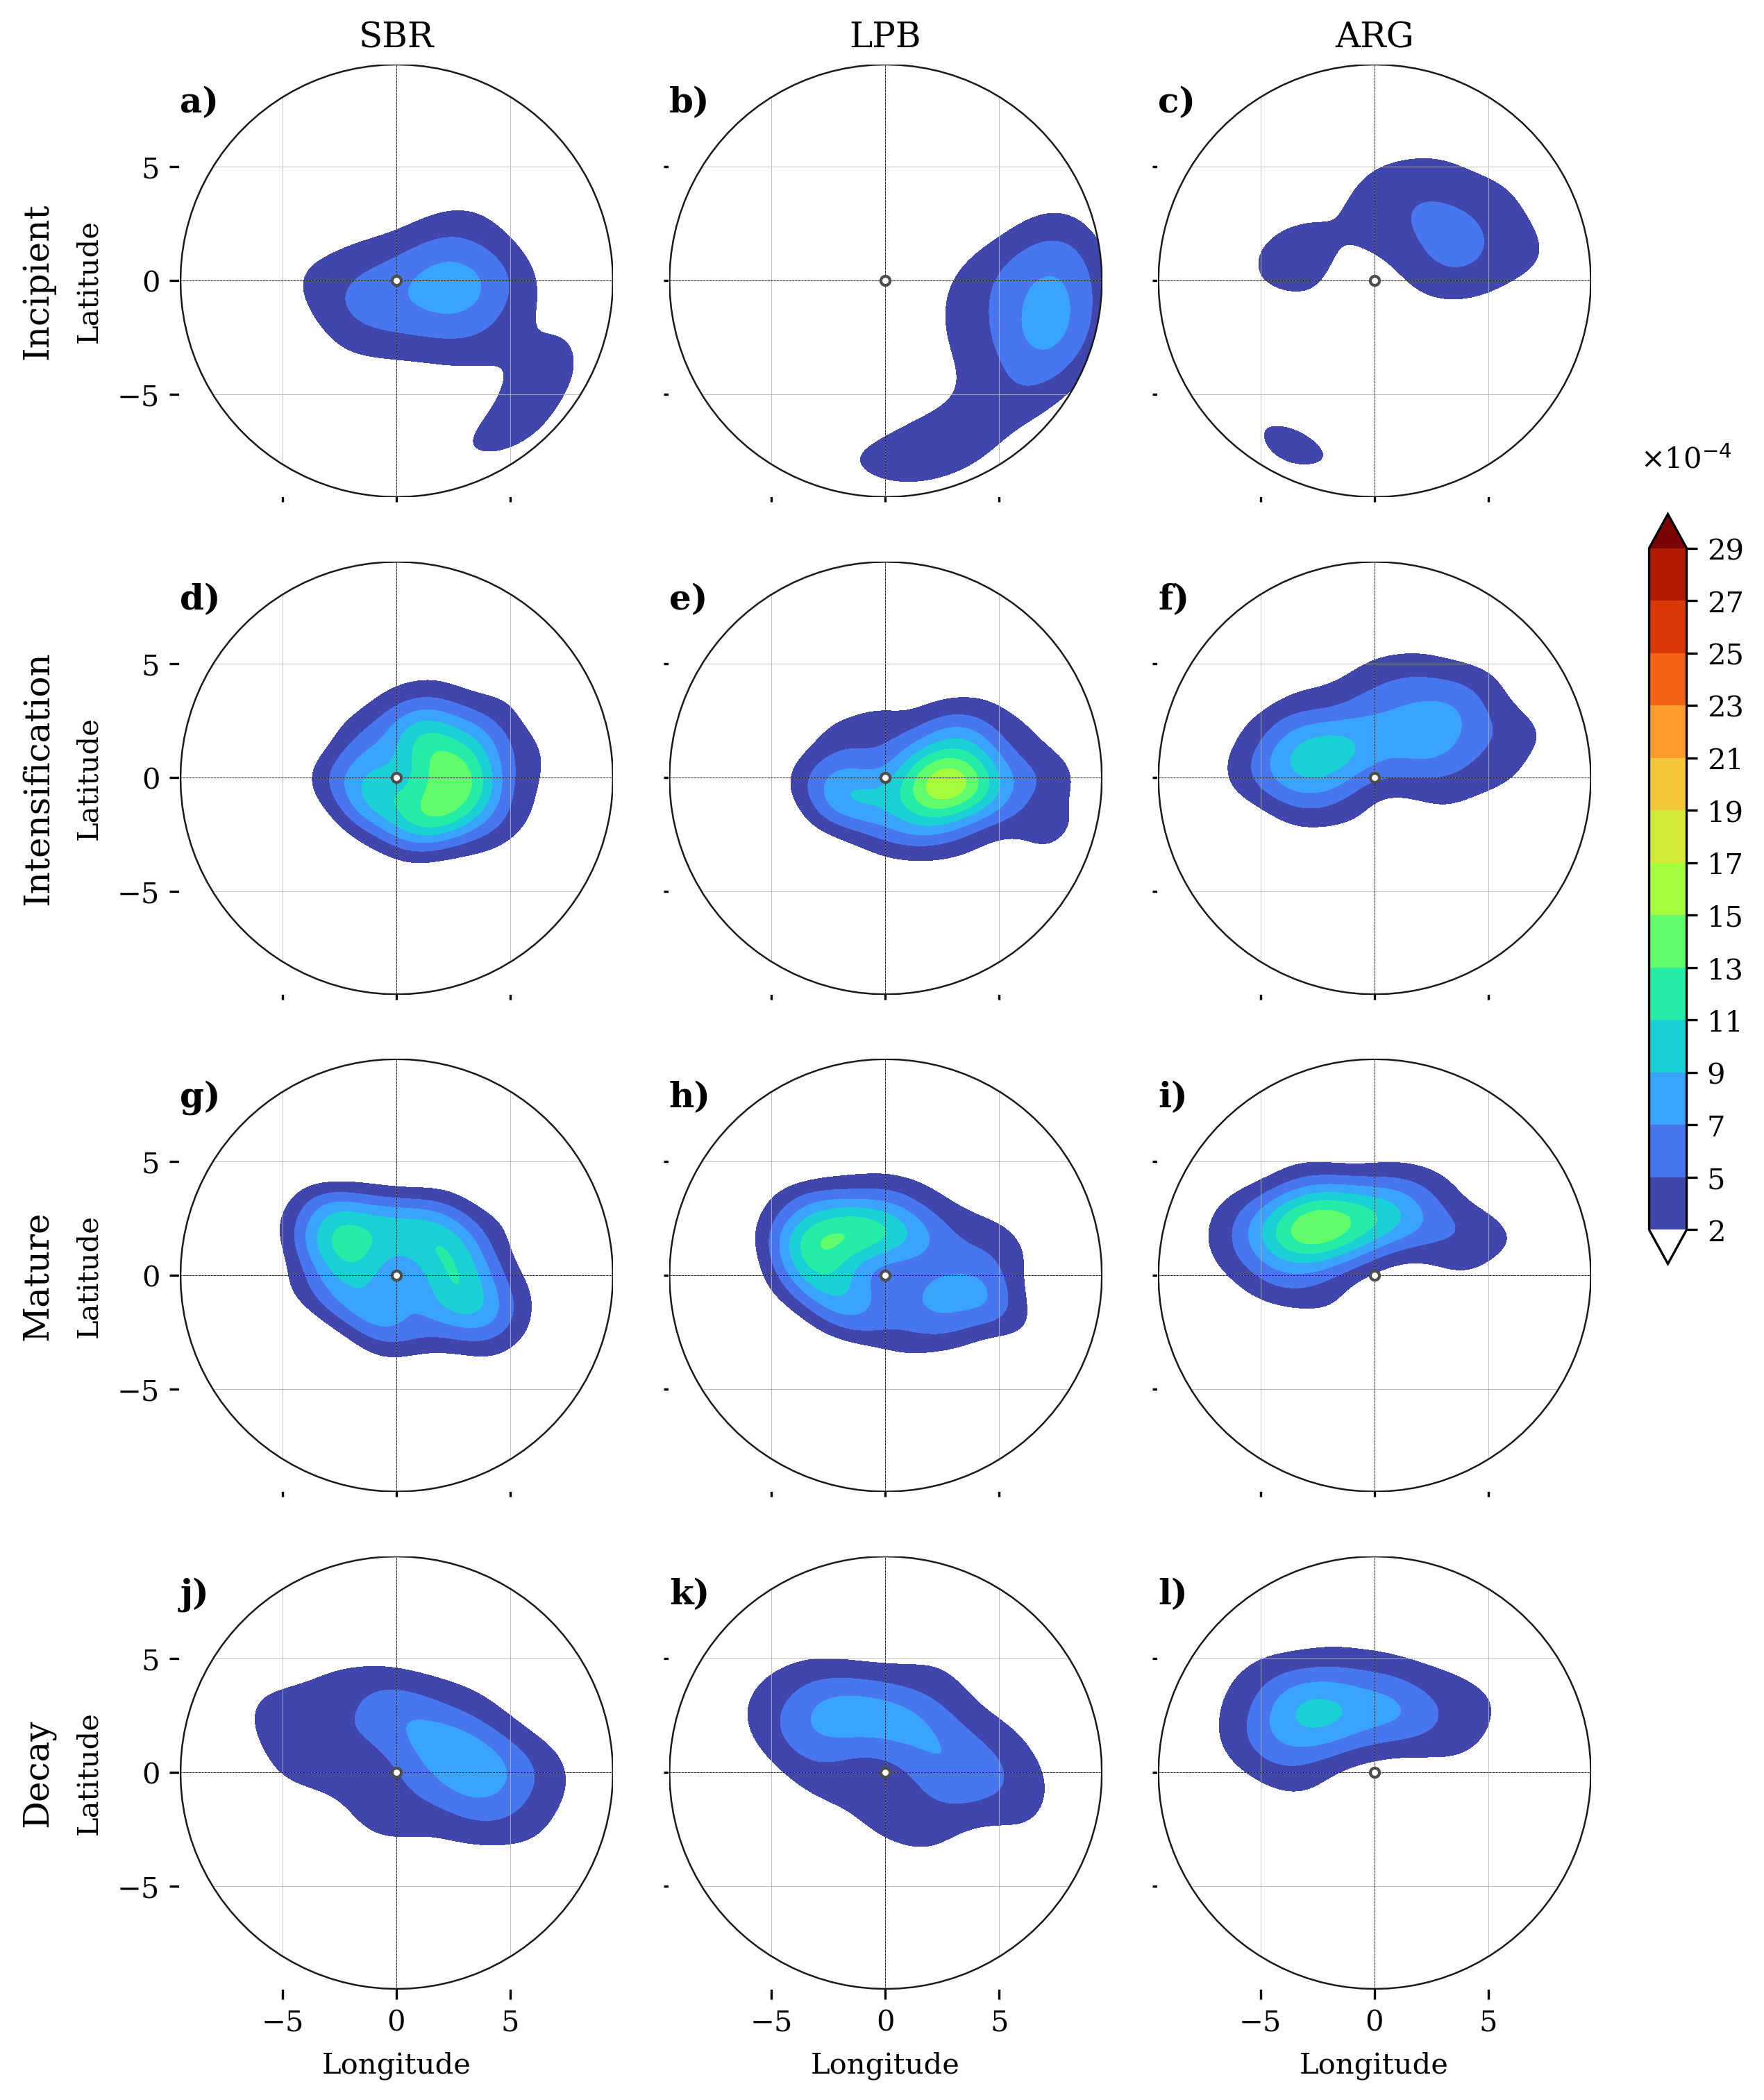
\includegraphics[width=\textwidth]{images/w10/kde_wind10_global_fasesxreg.png}
\caption[PDF espacial de vento máximo a 10 metros (População Global)]{Estimação de densidade espacial bidimensional (PDFe; Seção~\ref{subsec:kde_localizacion}) da localização dos máximos de magnitude de vento a 10~metros para a População Global. As colunas separam as regiões de ciclogênese (SBR, LPB, ARG) e as linhas indicam as fases evolutivas (Ic, It, M, D). O domínio está centrado no ciclone ($0^{\circ}, 0^{\circ}$).}
\label{fig:kde_wind_global}
\end{figure}

A Figura~\ref{fig:kde_wind_global} apresenta a densidade espacial da localização dos máximos de vento no domínio centrado no ciclone de $20^{\circ} \times 20^{\circ}$ (Seção~\ref{sec:procesamiento_lagrangiano}).
As distribuições são amplas e com gradientes suaves, e sua densidade máxima é menor do que a de p90 sobretudo na maturidade, nas três regiões ($11$--$15$ contra $19$--$27\times10^{-4}$). Nas demais fases as diferenças são menores e não seguem um sentido único. Em cinco dos nove casos a População Global chega a apresentar maior densidade, na fase incipiente de LPB e ARG, na intensificação de LPB e no decaimento de SBR e ARG.
Essa dispersão é a esperada em uma população heterogênea, já que a detecção por vorticidade também inclui centros móveis e menos profundos que a detecção por pressão omite \citep{sinclair1994objective}.

Na População Global, o núcleo de máxima densidade se localiza a leste do centro durante as fases incipiente e intensificação em SBR e LPB, e no quadrante noroeste durante a maturidade nas três regiões. Em ARG, esse deslocamento para o noroeste já ocorre durante a intensificação.
Na fase incipiente (Ic; painéis a, b e~c), as zonas de maior densidade abrangem áreas extensas e assimétricas, com o núcleo no setor leste (nordeste em ARG), o que concorda com sistemas que ainda não organizaram uma circulação fechada (Seção~\ref{subsec:tb_fases}).
Esse padrão é coerente com o observado por \citet{dejesus2021multimodel} nas reanálises, em que os ventos mais fortes em 1000~hPa ocupam o setor quente (nordeste no HS) do ciclone incipiente, embora sua amostra se restrinja às ciclogêneses mais intensas (quartil superior de vorticidade inicial) e seus compostos não estejam centrados no ciclone.
Durante a intensificação (It; painéis d, e e~f), as distribuições se tornam mais compactas e próximas do centro. Em SBR (d) e LPB (e) o núcleo permanece a leste, com a maior densidade dessa fase em LPB (${\approx}$\,15--17\,$\times10^{-4}$), enquanto em ARG (f) se localiza a oeste-noroeste e apresenta uma distribuição mais alongada em sentido zonal.
Na maturidade (M; painéis g, h e~i), o foco principal se situa no quadrante noroeste nas três regiões, com densidades de ${\approx}$\,11--15\,$\times10^{-4}$, e as diferenças regionais são discutidas a seguir.
No decaimento (D; painéis j, k e~l), as densidades diminuem até valores próximos aos da fase incipiente, e a localização do núcleo varia entre regiões, a leste-nordeste em SBR e a noroeste em LPB e ARG.

Na maturidade, ARG (i) apresenta um único núcleo no noroeste (${\approx}$\,13--15\,$\times10^{-4}$), enquanto SBR (g) e LPB (h) mostram um foco principal no noroeste e outro secundário a leste ou sudeste, com densidades máximas de ${\approx}$\,11--13\,$\times10^{-4}$ em SBR e ${\approx}$\,13--15\,$\times10^{-4}$ em LPB. Essa ordem regional não se repete na magnitude do vento (Seção~\ref{sec:pdf_wind10}), onde LPB e ARG apresentam os picos de densidade mais altos e SBR a distribuição mais larga, o que indica que a região que mais concentra a localização de seus máximos não é a que mais concentra sua intensidade.
Em ARG, esse padrão seria compatível com a advecção térmica e a perturbação topográfica andina, e em SBR e LPB com a advecção de ar quente e úmido (Seção~\ref{sec:tb_regiones}).

A dispersão da População Global reflete também a variabilidade na distância entre o centro e os ventos máximos. Em ciclones subtropicais do Atlântico Sul, \citet{gozzo2014subtropical} e \citet{cardoso2020wind} situam esses máximos entre 300 e 450~km e entre 400 e 500~km do centro, respectivamente, escalas que servem de referência ainda que não correspondam à população de ETCs aqui estudada. Essa heterogeneidade justifica separar os ciclones por intensidade (Seção~\ref{subsec:subconjuntos_intensidad}) e é coerente com o apontado por \citet{corner2025classification} para ciclones do Atlântico Norte e Europa, onde nem a pressão mínima nem a vorticidade máxima se relacionam bem com os impactos do ciclone, devido a estruturas de mesoescala que modulam o campo de vento. A seção seguinte analisa a localização dos máximos nos ciclones intensos, com essa população como referência.

\subsection{Subconjunto de ciclones intensos p90}\label{sec:kde_espacial_p90}

\begin{figure}[htbp]
\centering
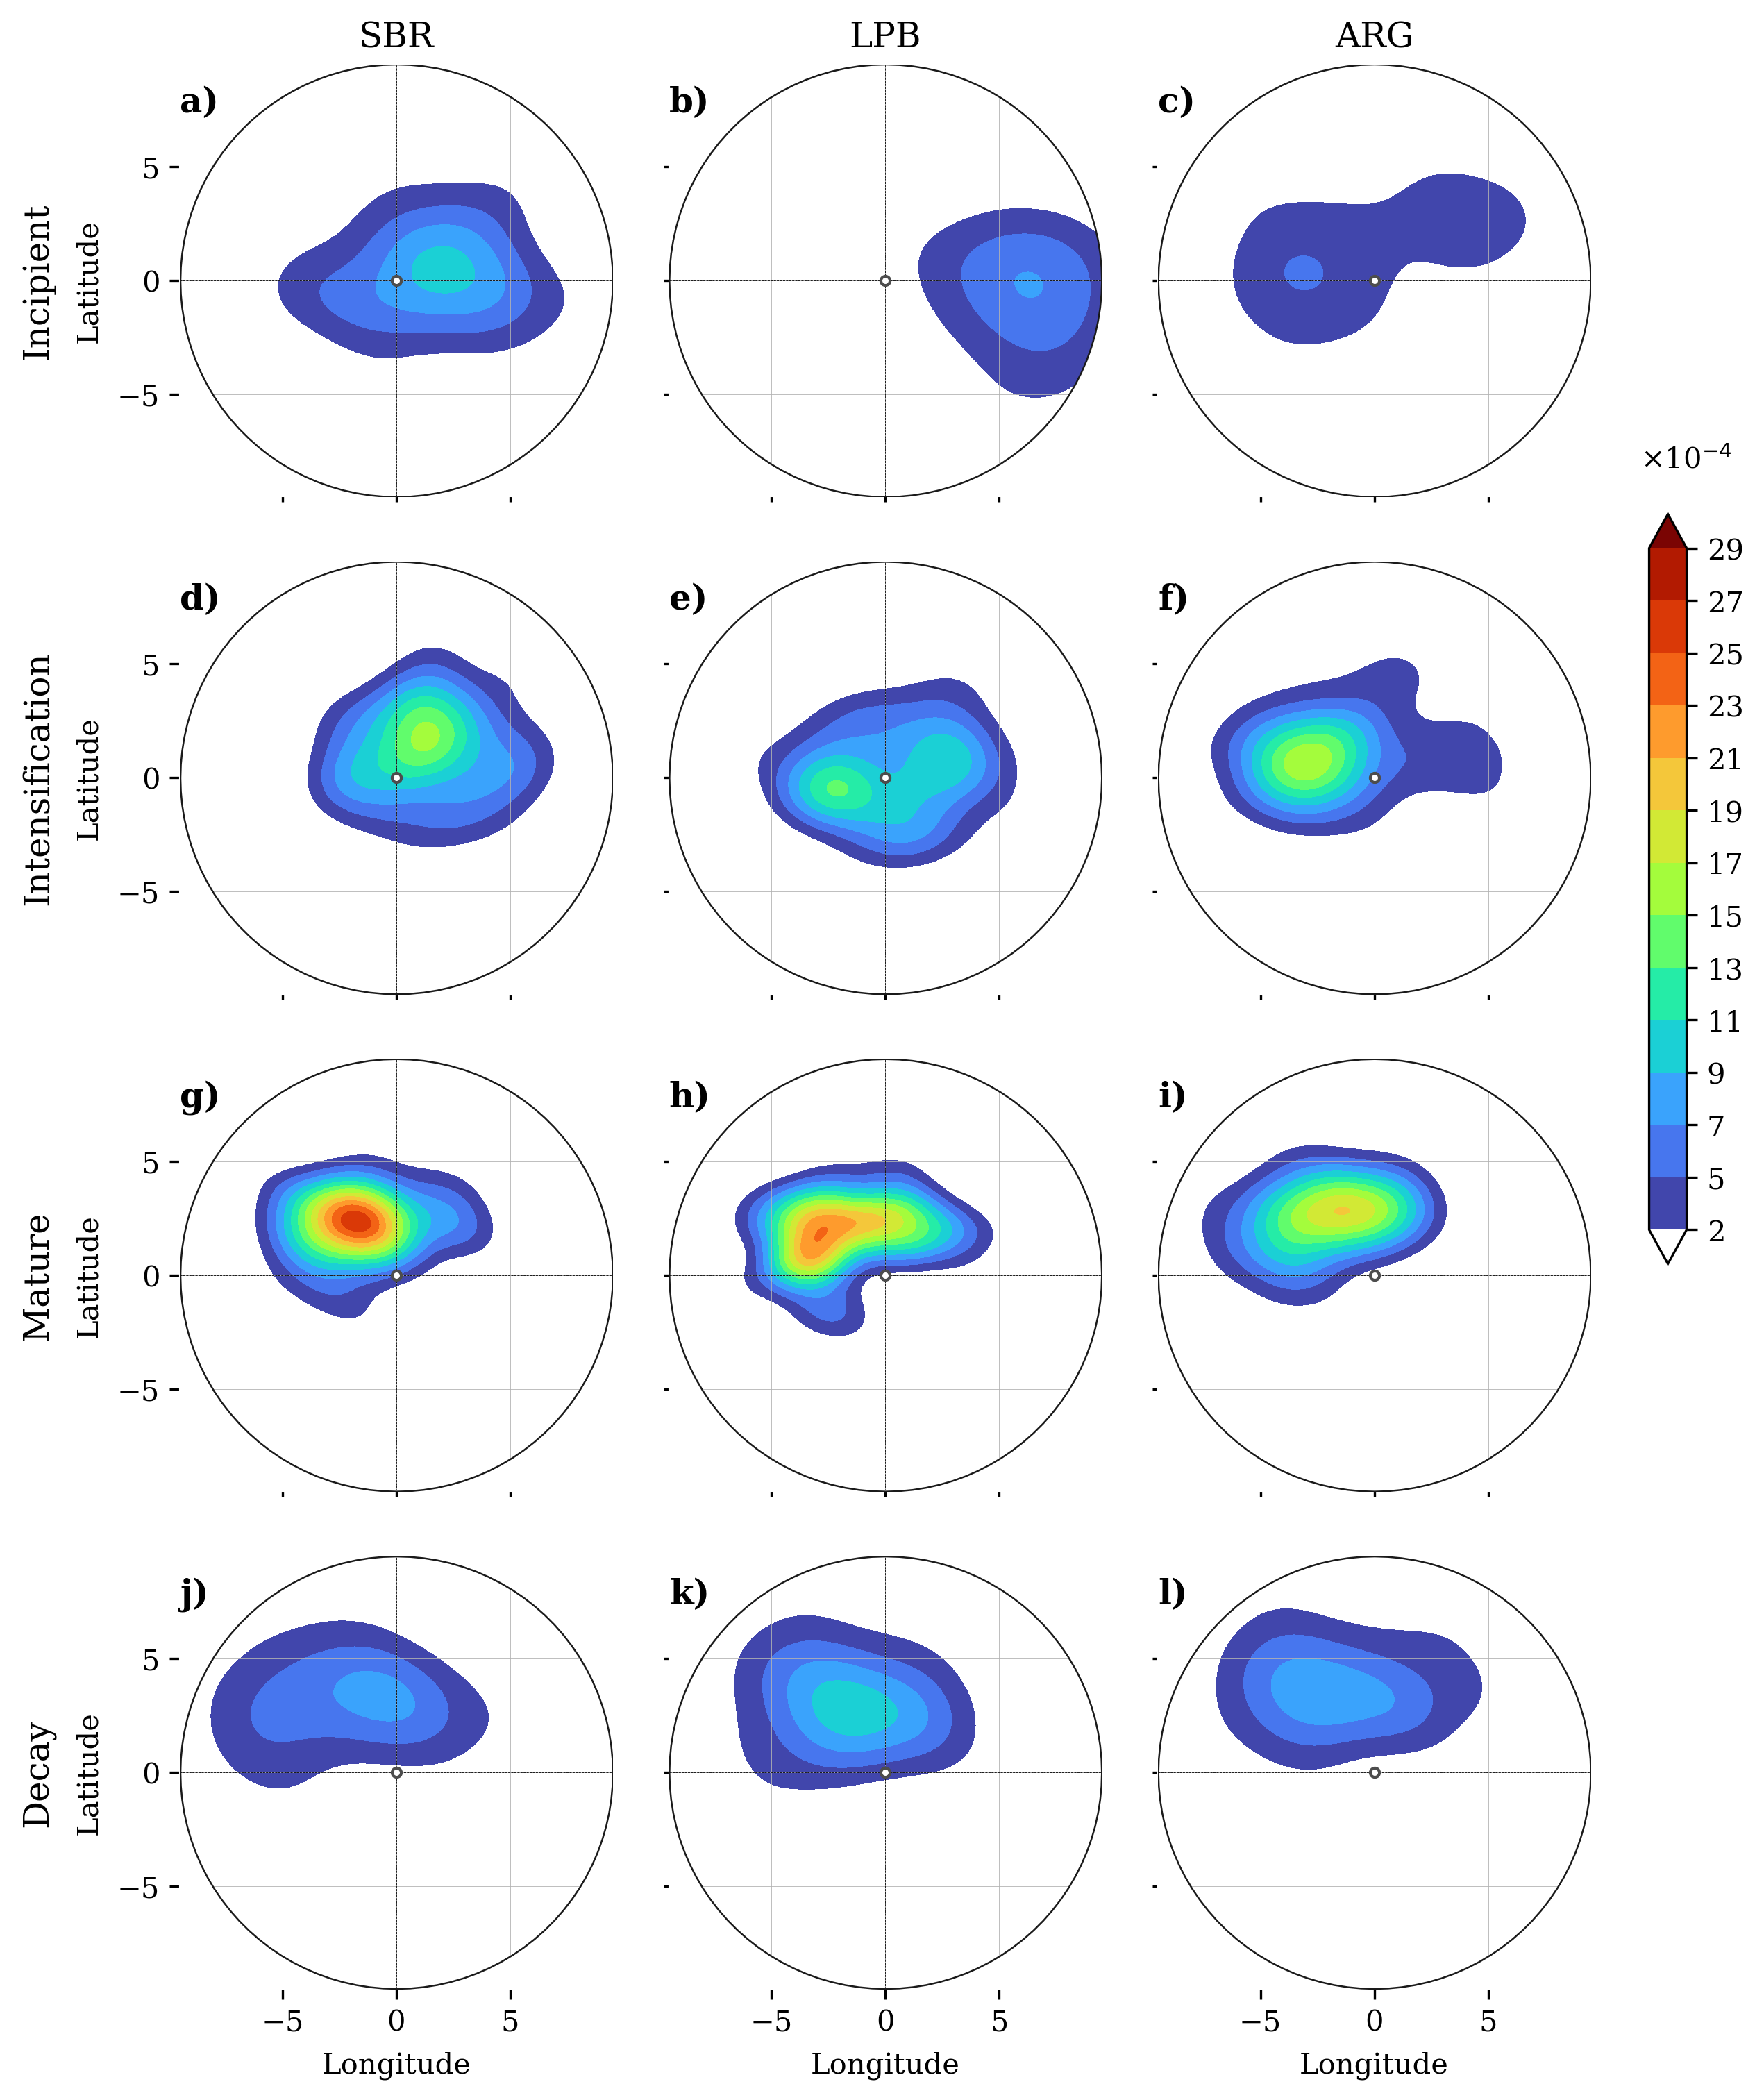
\includegraphics[width=\textwidth]{images/w10/kde_wind10_p90_fasesxreg.png}
\caption[PDF espacial de vento máximo a 10 metros (subconjunto p90)]{Estimação de densidade espacial bidimensional (PDFe; Seção~\ref{subsec:kde_localizacion}) da localização dos máximos de magnitude de vento a 10~metros para o subconjunto de ciclones intensos. O formato, domínio centrado no ciclone, fases evolutivas e escala de densidade ($10^{-4}$) são idênticos aos apresentados na Figura~\ref{fig:kde_wind_global} para permitir a comparação estrutural direta das assimetrias de densidade.}
\label{fig:kde_wind_p90}
\end{figure}

No subconjunto p90, a localização dos máximos se concentra progressivamente em um quadrante preferencial à medida que o ciclone evolui (Figura~\ref{fig:kde_wind_p90}).

Na fase incipiente (Ic; painéis a, b e~c), as três regiões apresentam densidades baixas e sem uma zona preferencial definida, de forma semelhante à População Global. Na intensificação (It; painéis d, e e~f), os núcleos começam a se deslocar para o oeste. Em SBR (d), o núcleo se localiza a nordeste e próximo do centro, mais a oeste do que na fase incipiente; em LPB (e), o núcleo principal se situa a oeste-sudoeste, com um núcleo secundário de menor densidade a leste; e em ARG (f), o núcleo se mantém a oeste do centro, como na fase incipiente, mas sua densidade aumenta de $5$--$7$ para $15$--$17\times10^{-4}$.
Na maturidade (M; painéis g, h e~i) forma-se um núcleo de alta densidade no quadrante noroeste, entre $-1^{\circ}$ e $-3^{\circ}$ de longitude e entre $+1.5^{\circ}$ e $+3^{\circ}$ de latitude em relação ao centro.
A densidade máxima é de 25--27\,$\times 10^{-4}$ em SBR (g), ${\approx}$\,23--25\,$\times 10^{-4}$ em LPB (h) e ${\approx}$\,19--21\,$\times 10^{-4}$ em ARG (i), cujo núcleo é menos compacto. Essa ordem regional não se repete na magnitude do vento (Seção~\ref{sec:pdf_wind10}), onde LPB e ARG apresentam os picos de densidade mais altos e SBR a distribuição mais larga, o que indica que a região que mais concentra a localização de seus máximos não é a que mais concentra sua intensidade.
No decaimento (D; painéis j, k e~l), o núcleo permanece no noroeste nas três regiões, enquanto na População Global o de SBR se localizava a leste-nordeste.

Essa alta concentração no noroeste é o traço espacial mais distintivo do vento nos ciclones p90 durante a maturidade, comum às três regiões de estudo.
Em ciclones do Hemisfério Norte documentam-se padrões análogos, com os ventos extremos associados ao \textit{sting jet}, que desce na zona de fratura frontal, e ao jato da cinta transportadora fria (CCB, \textit{cold conveyor belt}), situado abaixo e atrás dele \citep{clark2005sting, clark2018sting}, duas estruturas difíceis de distinguir em superfície por sua proximidade no espaço e no tempo \citep{eisenstein2023identification}. Pela inversão da circulação entre hemisférios, esse setor corresponde ao quadrante noroeste no Hemisfério Sul.
Com a mesma lógica, o máximo de vento que \citet{rudeva2011composite} localizam no setor sudoeste de ciclones do Atlântico Norte, a meia distância entre o centro e a borda do sistema, corresponderia ao quadrante noroeste no Hemisfério Sul, embora essa correspondência se baseie na simetria entre hemisférios e não em uma comparação direta.
De forma semelhante, \citet{priestley2022improved} situam os máximos do vento relativo ao sistema a 850~hPa associados ao CCB a ${\sim}$3--3.5$^{\circ}$ do centro e no flanco posterior de ciclones do Hemisfério Norte, uma distância comparável à do núcleo aqui identificado, e \citet{laurila2021characteristics} mostram que, nas tempestades de vento do norte da Europa, as rajadas mais intensas se deslocam do setor quente para detrás da frente fria ao longo da evolução do ciclone. Em um composto dos 100 ciclones mais intensos do Atlântico Norte, \citet{gentile2025response} descrevem uma sequência semelhante para o vento a 10~m, que se localiza no setor quente e em direção ao equador durante as primeiras etapas, e detrás do centro, no setor frio e ainda em direção ao equador, à medida que o ciclone se intensifica, o que no Hemisfério Sul corresponderia a um deslocamento para o noroeste.

No Atlântico Sul, \citet{gramcianinov2023impact} constatam que as ondas extremas associadas a ciclones ocorrem principalmente nos setores oeste e noroeste do ciclone, dominados pelo CCB, exceto em SBR durante o verão, quando predomina o setor leste, influenciado pelo WCB.
Em contraste, o composto de \citet{catto2010climate} sobre os 100 ciclones mais intensos do Hemisfério Norte no inverno situou parte dos ventos mais intensos a 925~hPa (${39.1 \pm 3.5}$~m\,s$^{-1}$, a ${5.1^{\circ} \pm 2.7^{\circ}}$ do centro) no setor quente onde se localiza o WCB, o que no Hemisfério Sul corresponderia ao quadrante nordeste. Essa diferença em relação ao núcleo noroeste de p90 poderia refletir o nível analisado (925~hPa contra 10~m) e o fato de que seu composto é construído no instante de máxima intensidade de cada ciclone, sem separar fases.
Fora do Atlântico Norte, a climatologia global de \citet{gray2024global}, que identifica precursores de \textit{sting jet} nos três oceanos durante 43 invernos, mostra que ciclones com esses precursores também ocorrem no Hemisfério Sul, embora com menor frequência (${\sim}$15\% do decil superior de intensidade, contra ${\sim}$27\% no Hemisfério Norte).

A concentração desse núcleo poderia estar relacionada ao transporte de momento em direção à superfície. Próximo à frente fria desenvolvem-se correntes descendentes que transportam momento horizontal de níveis altos para níveis baixos, e em climatologias do Hemisfério Norte essas correntes são cerca de 15\% mais frequentes no setor sudoeste do ciclone, que corresponde ao noroeste no Hemisfério Sul \citep{hyeok2024extrem}. Além disso, segundo \citet{martinez2014cold} (Seção~\ref{subsec:tb_modelos}), os ventos mais intensos na parte posterior do núcleo estão associados ao CCB e ao \textit{sting jet}, e o jato de baixo nível do CCB se intensifica pelo aumento de vorticidade potencial gerado pelo aquecimento diabático sob a ascensão do WCB \citep{schemm2014linkage}.

\citet{gentile2023observed} mostram também que, em ciclones maduros, o CCB ocorre no setor frio com camadas limite mais profundas e instáveis, o que favorece a mistura de ar de alta velocidade em direção à superfície e seria compatível com a concentração observada na PDFe. \citet{stankovic2025surface} reportam extremos de vento em superfície mais intensos no Hemisfério Norte do que no oceano Austral, associados a uma maior baroclinicidade em níveis médios, o que deve ser considerado ao comparar as magnitudes aqui obtidas com estudos desse hemisfério.

Deve-se considerar que o ERA5 pode subestimar a intensidade do vento por sua resolução. Ao não resolver explicitamente as estruturas de mesoescala, tende a subestimar as magnitudes extremas \citep{hodges2011comparison}, em torno de 10\% para o vento dos ciclones mais intensos segundo \citet{chen2024evaluation} (Seção~\ref{sec:datos_era5}), o que deve ser levado em conta ao interpretar os valores absolutos.

Uma referência observacional da magnitude que o vento pode alcançar nessas estruturas é o caso documentado por \citet{shapiro1990life}. Durante a fase de seclusão quente de um ETC profundo do Atlântico Norte (pressão central ${\sim}935$~hPa), medições de aeronave registraram velocidades de ${\sim}$40~m\,s$^{-1}$ a cerca de 300~m de altitude. Embora não correspondam ao vento a 10~m, que é menor por efeito do atrito, esses valores sugerem que as caudas de até 30~m\,s$^{-1}$ de p90 no ERA5 (Seção~\ref{sec:pdf_wind10}) poderiam estar subestimadas.

\citet{gray2020prototype} documentam um caso próximo à superfície, a tempestade Brendan (Reino Unido, janeiro de 2020; aprofundamento de 49~hPa em 24~h), no qual o dispersômetro ASCAT registrou ventos equivalentes a 10~m superiores a 55~nós (${\sim}28$~m\,s$^{-1}$) ao sul do centro, na zona de fratura frontal apontada como precursora de \textit{sting jet}, embora nessas observações o CCB e o \textit{sting jet} não possam ser distinguidos. Pela inversão entre hemisférios, essa zona corresponde ao lado norte do centro no Hemisfério Sul, e a magnitude registrada é comparável às caudas de p90 aqui obtidas.

Em conjunto, esses resultados mostram que a intensidade de um ciclone está associada ao seu padrão espacial. Os ciclones intensos das três regiões tendem a concentrar seus máximos de vento a 10~m a uma distância e em um quadrante preferenciais em relação ao centro, o que sugere incorporar a localização, e não apenas a magnitude, ao avaliar os impactos do vento associados a esses sistemas.
%%%%%%%%%%%%%
% --- SEÇÃO: PADRÕES DOMINANTES DE VARIABILIDADE (EOF) - VENTO A 10 METROS,
\section{Organização estrutural: Análise EOF}\label{sec:eof_wind10}
\subsection{Fracionamento de variância}\label{sec:var_exp_wind10}
\begin{figure}[htbp]
\centering
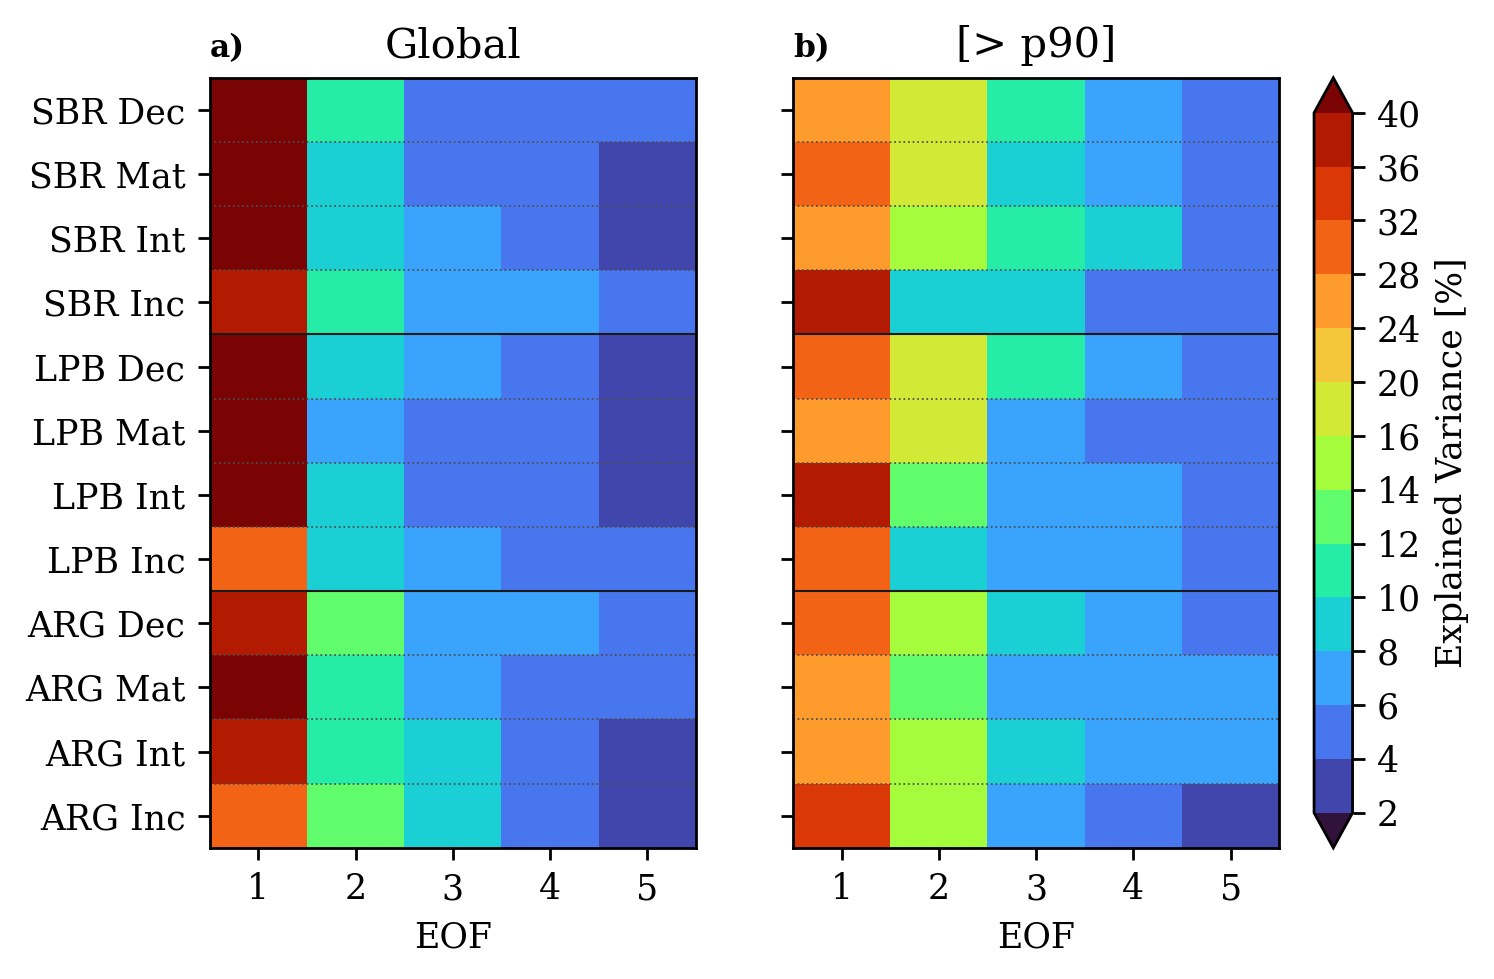
\includegraphics[width=0.8\textwidth]{images/w10/all_expvar_wind10_mean2times.png}
\caption[Variância explicada pelos primeiros cinco modos (EOF1--EOF5) de vento a 10~m]{Fracionamento da variância espacial total contida nos primeiros cinco modos dominantes (EOF1 a EOF5) do vento a 10~metros, obtida mediante o procedimento descrito na Seção~\ref{subsec:eof_univariado}. Contrasta-se a distribuição da variância da População Global com o subconjunto de intensidade p90 ao longo do ciclo de vida para cada região de ciclogênese.}
\label{fig:var_exp_wind10}
\end{figure}

A Figura~\ref{fig:var_exp_wind10} resume a variância explicada pelos cinco primeiros modos (EOF1 a EOF5) na População Global (painel~a) e em p90 (painel~b). Na População Global, EOF1 domina sobre os modos secundários em todas as regiões e fases, com valores máximos na maturidade (57.4\% em SBR e 57.1\% em LPB) e uma queda abrupta em direção ao EOF2. Os valores mais baixos são registrados em ARG (entre 30.9\% e 43.3\%) e em LPB durante a fase incipiente (31.9\%). Isso indica que, na População Global, a variabilidade do vento em superfície se concentra em um único padrão espacial, compatível com um gradiente de grande escala como o fluxo sinótico de fundo (Seção~\ref{subsec:eof_univariado}).

Em p90, EOF1 não supera 37.6\% em nenhuma região nem fase, com um mínimo de 25.4\% em ARG durante a intensificação, e a variância se distribui entre vários modos, com maior peso de EOF2 e EOF3. Segundo \citet{hannachi2007empirical}, o espectro de autovalores indica como a variância se distribui segundo a escala espacial, e quando os autovalores são próximos, os padrões correspondentes podem se misturar e devem ser interpretados com cautela. Nos ciclones intensos, a maior complexidade do vórtice, com frentes mais marcadas, jatos de baixo nível e seclusão quente (Seção~\ref{subsec:tb_modelos}), poderia explicar que sejam necessários vários modos (EOF2--EOF5) para representar a variabilidade do campo.

Esses resultados indicam que um ciclone intenso não é uma versão amplificada de um ciclone ordinário. Como em p90 a variância se distribui entre vários modos, descrever seus ventos a partir dos padrões da população média poderia não representar adequadamente a assimetria nem a localização de seus máximos.
%%%%%%%
\subsection{EOF1 na População Global}\label{subsec:eof1_wind10_global}

\begin{figure}[htbp]
\centering
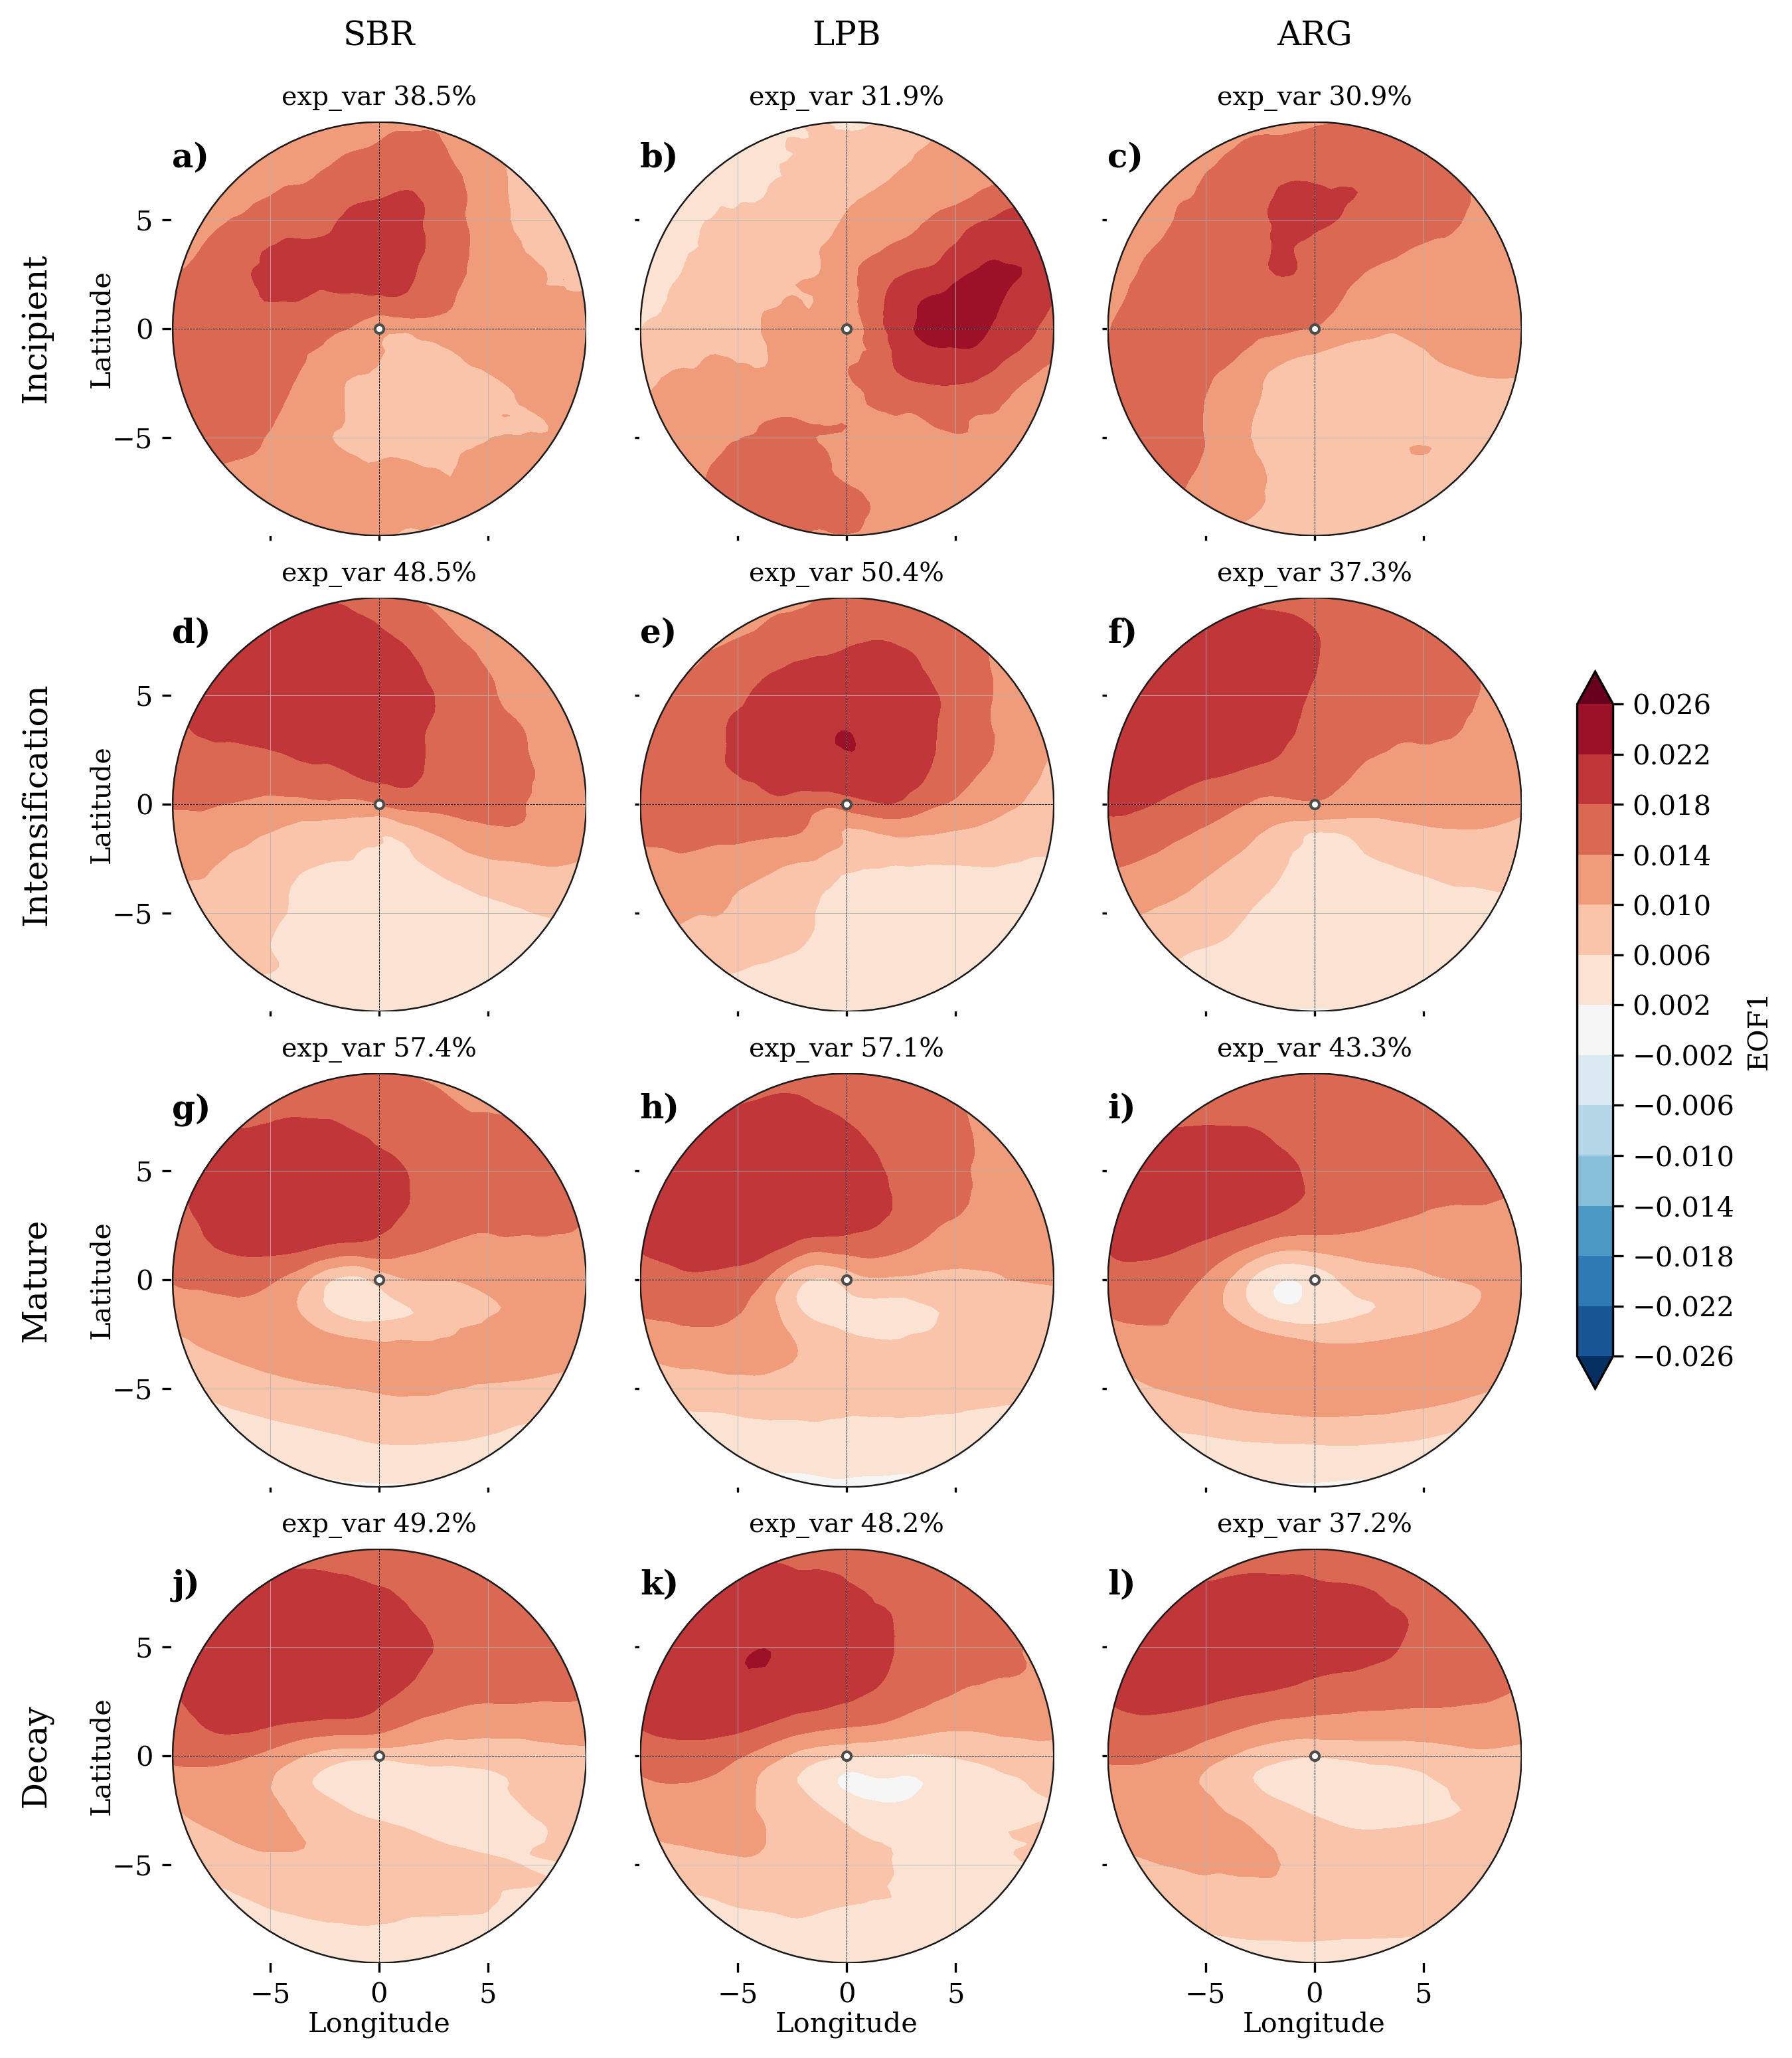
\includegraphics[width=\textwidth]{images/w10/pca1_wind10_global_fasesxreg.png}
\caption[EOF1 da magnitude do vento a 10 metros (População Global)]{Primeiro modo espacial (EOF1) da magnitude do vento a 10~metros para a População Global de referência, derivado da análise descrita na Seção~\ref{subsec:eof_univariado}. Os painéis (a--c) correspondem à fase incipiente (Ic) para as regiões SBR, LPB e ARG, respectivamente; (d--f) à intensificação (It); (g--i) à maturidade (M); e (j--l) ao decaimento (D). O título de cada painel indica o percentual de variância explicada (\textit{exp\_var}) por esse modo dominante. As cores quentes (frias) representam anomalias positivas (negativas) da estrutura do vento relativo ao centro do ciclone em um domínio de $20^{\circ} \times 20^{\circ}$.}
\label{fig:eof1_wind10_global}
\end{figure}

A Figura~\ref{fig:eof1_wind10_global} apresenta o EOF1 do vento a 10~m no domínio centrado no ciclone, que explica entre 30.9\% (ARG incipiente) e 57.4\% (SBR maturidade) da variância (Seção~\ref{sec:var_exp_wind10}). O padrão é positivo em todo o domínio e forma um gradiente norte--sul de grande escala, com valores altos no setor norte ($+0.010$ a $+0.026$) e valores próximos de zero no sul e em torno do centro. Esse gradiente se define progressivamente desde a fase incipiente até a maturidade, quando alcança sua maior variância explicada em SBR (g, 57.4\%) e LPB (h, 57.1\%). LPB se desvia desse comportamento nas primeiras fases, com o núcleo positivo a leste do centro na fase incipiente (b) e próximo do centro na intensificação (e). No decaimento (j, k e~l), as três regiões apresentam valores altos a noroeste que diminuem em direção ao sudeste, com anomalias positivas fracas em quase todo o domínio.

A presença desse gradiente norte--sul desde a intensificação até a maturidade, junto com sua alta variância explicada, sugere que a variabilidade do vento nos ciclones depende em parte de sua interação com o fluxo zonal de fundo e com as variações do gradiente latitudinal de temperatura.
Em LPB, onde o padrão se desvia desse comportamento nas primeiras fases, \citet{gramcianinov2019properties} apontam que o desenvolvimento inicial é influenciado por uma baixa orográfica, o que poderia manter a variabilidade do vento próxima do centro e retardar o surgimento do gradiente norte--sul.

No decaimento, a circulação ciclônica se debilita e a variabilidade do vento passa a depender principalmente do fluxo zonal do entorno.
Esse padrão estabelece a referência de variabilidade do vento nos ETC para a comparação com os ciclones intensos e com a análise multivariada (Seção~\ref{sec:meof_prototipos}).
%%%%%%
\subsection{EOF1 no subconjunto p90}\label{subsec:eof1_wind10_p90}

\begin{figure}[htbp]
\centering
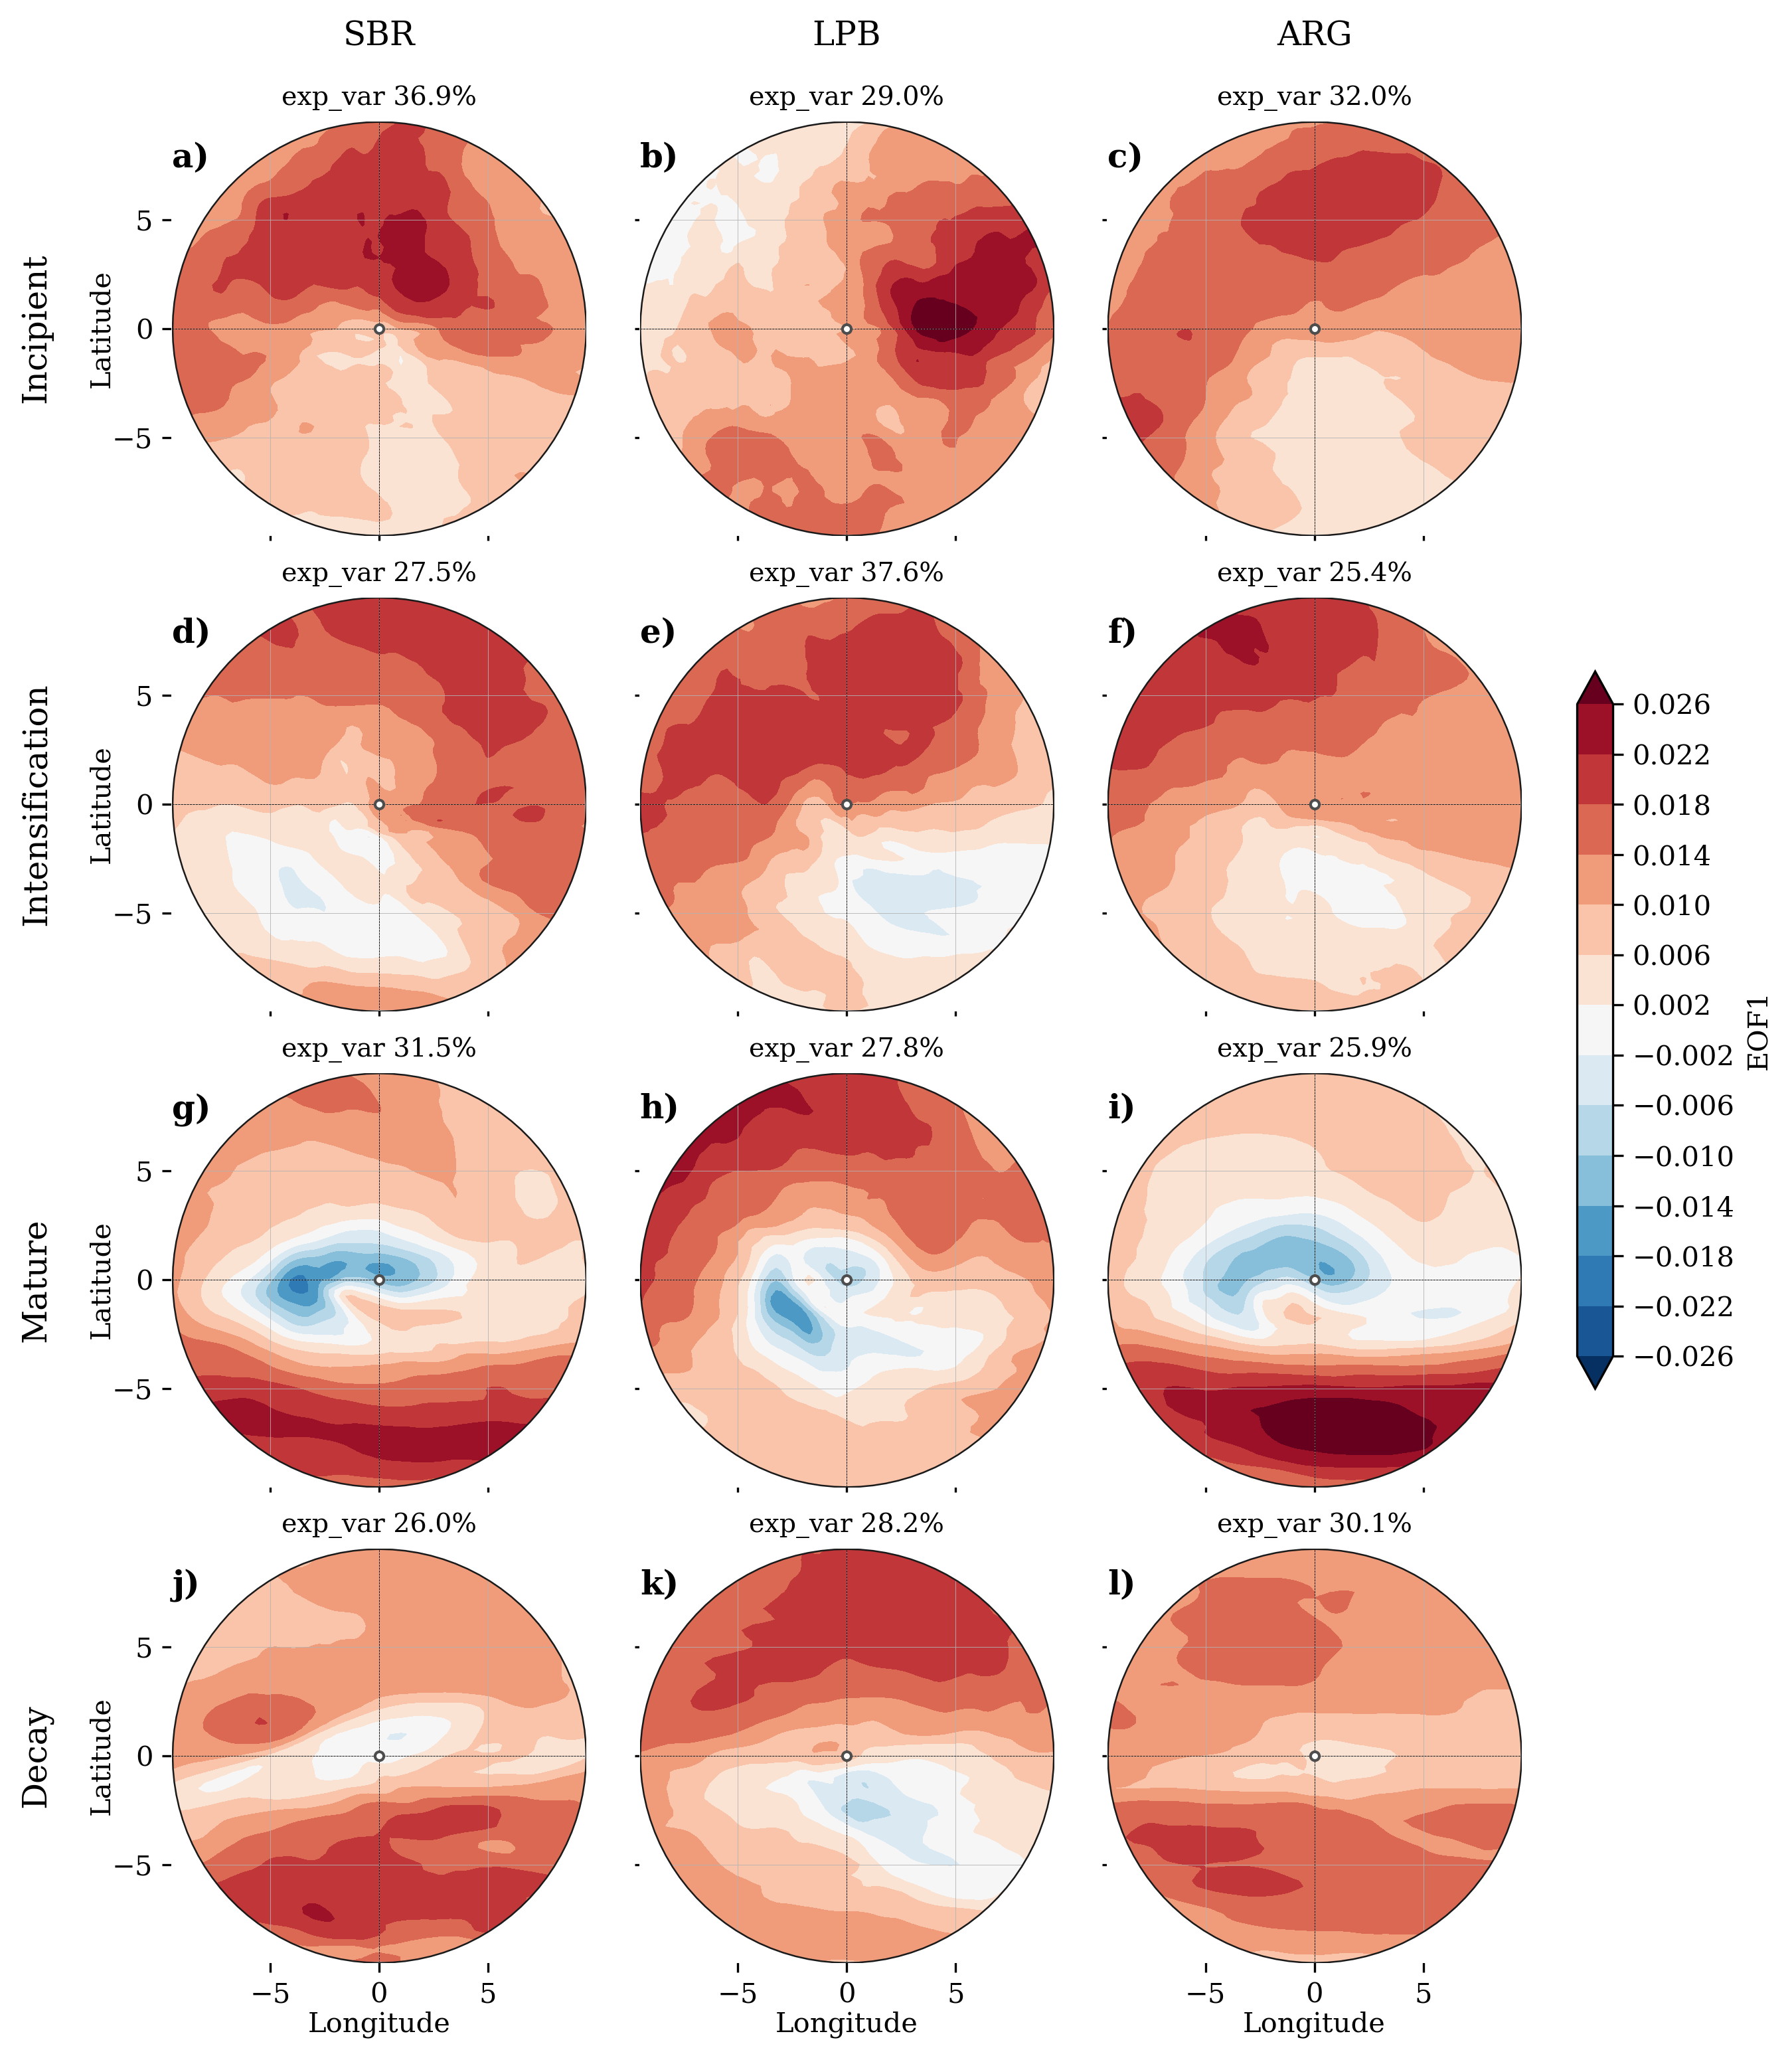
\includegraphics[width=\textwidth]{images/w10/pca1_wind10_p90_fasesxreg.png}
\caption[EOF1 da magnitude do vento a 10 metros (subconjunto p90)]{Primeiro modo espacial (EOF1) da magnitude do vento a 10~metros para o subconjunto de ciclones intensos (p90). A disposição dos painéis (a--l) por região de ciclogênese (colunas) e fase evolutiva (linhas) é idêntica à
Figura~\ref{fig:eof1_wind10_global}. Detalha-se a variância explicada (\textit{exp\_var}) em cada painel e a barra de cor padronizada para avaliar
as diferenças nos padrões espaciais dos ciclones intensos em relação à População Global.}
\label{fig:eof1_wind10_p90}
\end{figure}

Em p90, o EOF1 não amplifica o padrão da População Global, mas muda de forma. Sua variância explicada é menor (25.4--37.6\%) e o padrão apresenta estruturas mais localizadas do que o gradiente norte--sul de grande escala da Seção~\ref{subsec:eof1_wind10_global}.

Na fase incipiente (a, b e~c), as três regiões mostram padrões difusos, com anomalias positivas ao norte e nordeste e sem uma estrutura definida. Na intensificação (d, e e~f) aparece um gradiente norte--sul mais definido, com anomalias positivas ao norte, nordeste e noroeste e valores negativos fracos ao sul em SBR e LPB. ARG (f) apresenta os valores mais altos ($>+0.022$ no noroeste). A maior mudança ocorre na maturidade (g, h e~i), quando as três regiões desenvolvem um núcleo negativo compacto próximo do centro, rodeado de anomalias positivas ao norte e ao sul. Esse núcleo alcança valores de até $-0.022$ em SBR (g), a oeste do centro, e em LPB (h), onde se estende para o sudoeste, enquanto em ARG (i) é mais fraco. No decaimento (j, k e~l), o padrão perde definição e o domínio volta a ser majoritariamente positivo, com gradientes mais suaves, e apenas LPB mantém valores negativos fracos ao sul do centro.

Na maturidade, as anomalias se concentram próximo do núcleo, o que concorda com a distribuição da variância entre vários modos (Seção~\ref{sec:var_exp_wind10}). Nesses ciclones, o EOF1 deixa de descrever um gradiente sinótico extenso e passa a descrever a variabilidade próximo do núcleo, em posição e intensidade, o que sugere um maior peso da circulação de mesoescala em relação ao fluxo de fundo. Essa localização coincide com a zona onde a literatura situa o CCB e a fratura frontal (Seção~\ref{sec:kde_espacial_p90}), embora com o vento escalar disponível não seja possível distingui-la de outros mecanismos de escala semelhante, como o \textit{sting jet} ou a intrusão seca.

Em ARG durante a maturidade (i), as anomalias negativas em torno do centro são moderadas e a faixa positiva ao sul alcança os valores mais altos do domínio, padrão que poderia estar relacionado à seclusão quente (\textit{warm seclusion}; Seções~\ref{subsec:tb_modelos} e~\ref{subsec:tb_fases}).

Em conjunto, um ciclone intenso não é estruturalmente equivalente a um ciclone ordinário, já que sua dinâmica modifica a forma dos padrões de vento. Como apontam \citet{corner2025classification} e \citet{eisenstein2023identification}, a intensidade do vento em superfície não depende apenas da escala sinótica, mas também das estruturas de mesoescala.
%%%%%%%%
\subsection{Significância estatística}\label{subsec:res_significancia_madurez}

Para distinguir os sinais físicos das flutuações devidas à amostragem, avalia-se a significância estatística dos padrões espaciais mediante o método Bootstrap-t (Seção~\ref{subsec:bootstrap_significancia}), seguindo \citet{hesterberg2015bootstrap}. A análise se concentra na fase de maturidade, que apresenta o maior sinal dinâmico e é a de maior interesse para esta tese. A Figura~\ref{fig:xeof_madurez_global} mostra os três primeiros modos (EOF1--EOF3) e suas componentes principais (PC1--PC3) para a População Global na maturidade, e a Figura~\ref{fig:xeof_madurez_p90} apresenta a análise equivalente para p90. O hachurado indica as áreas significativas a 95\% de confiança.

\begin{figure}[htbp]
\centering
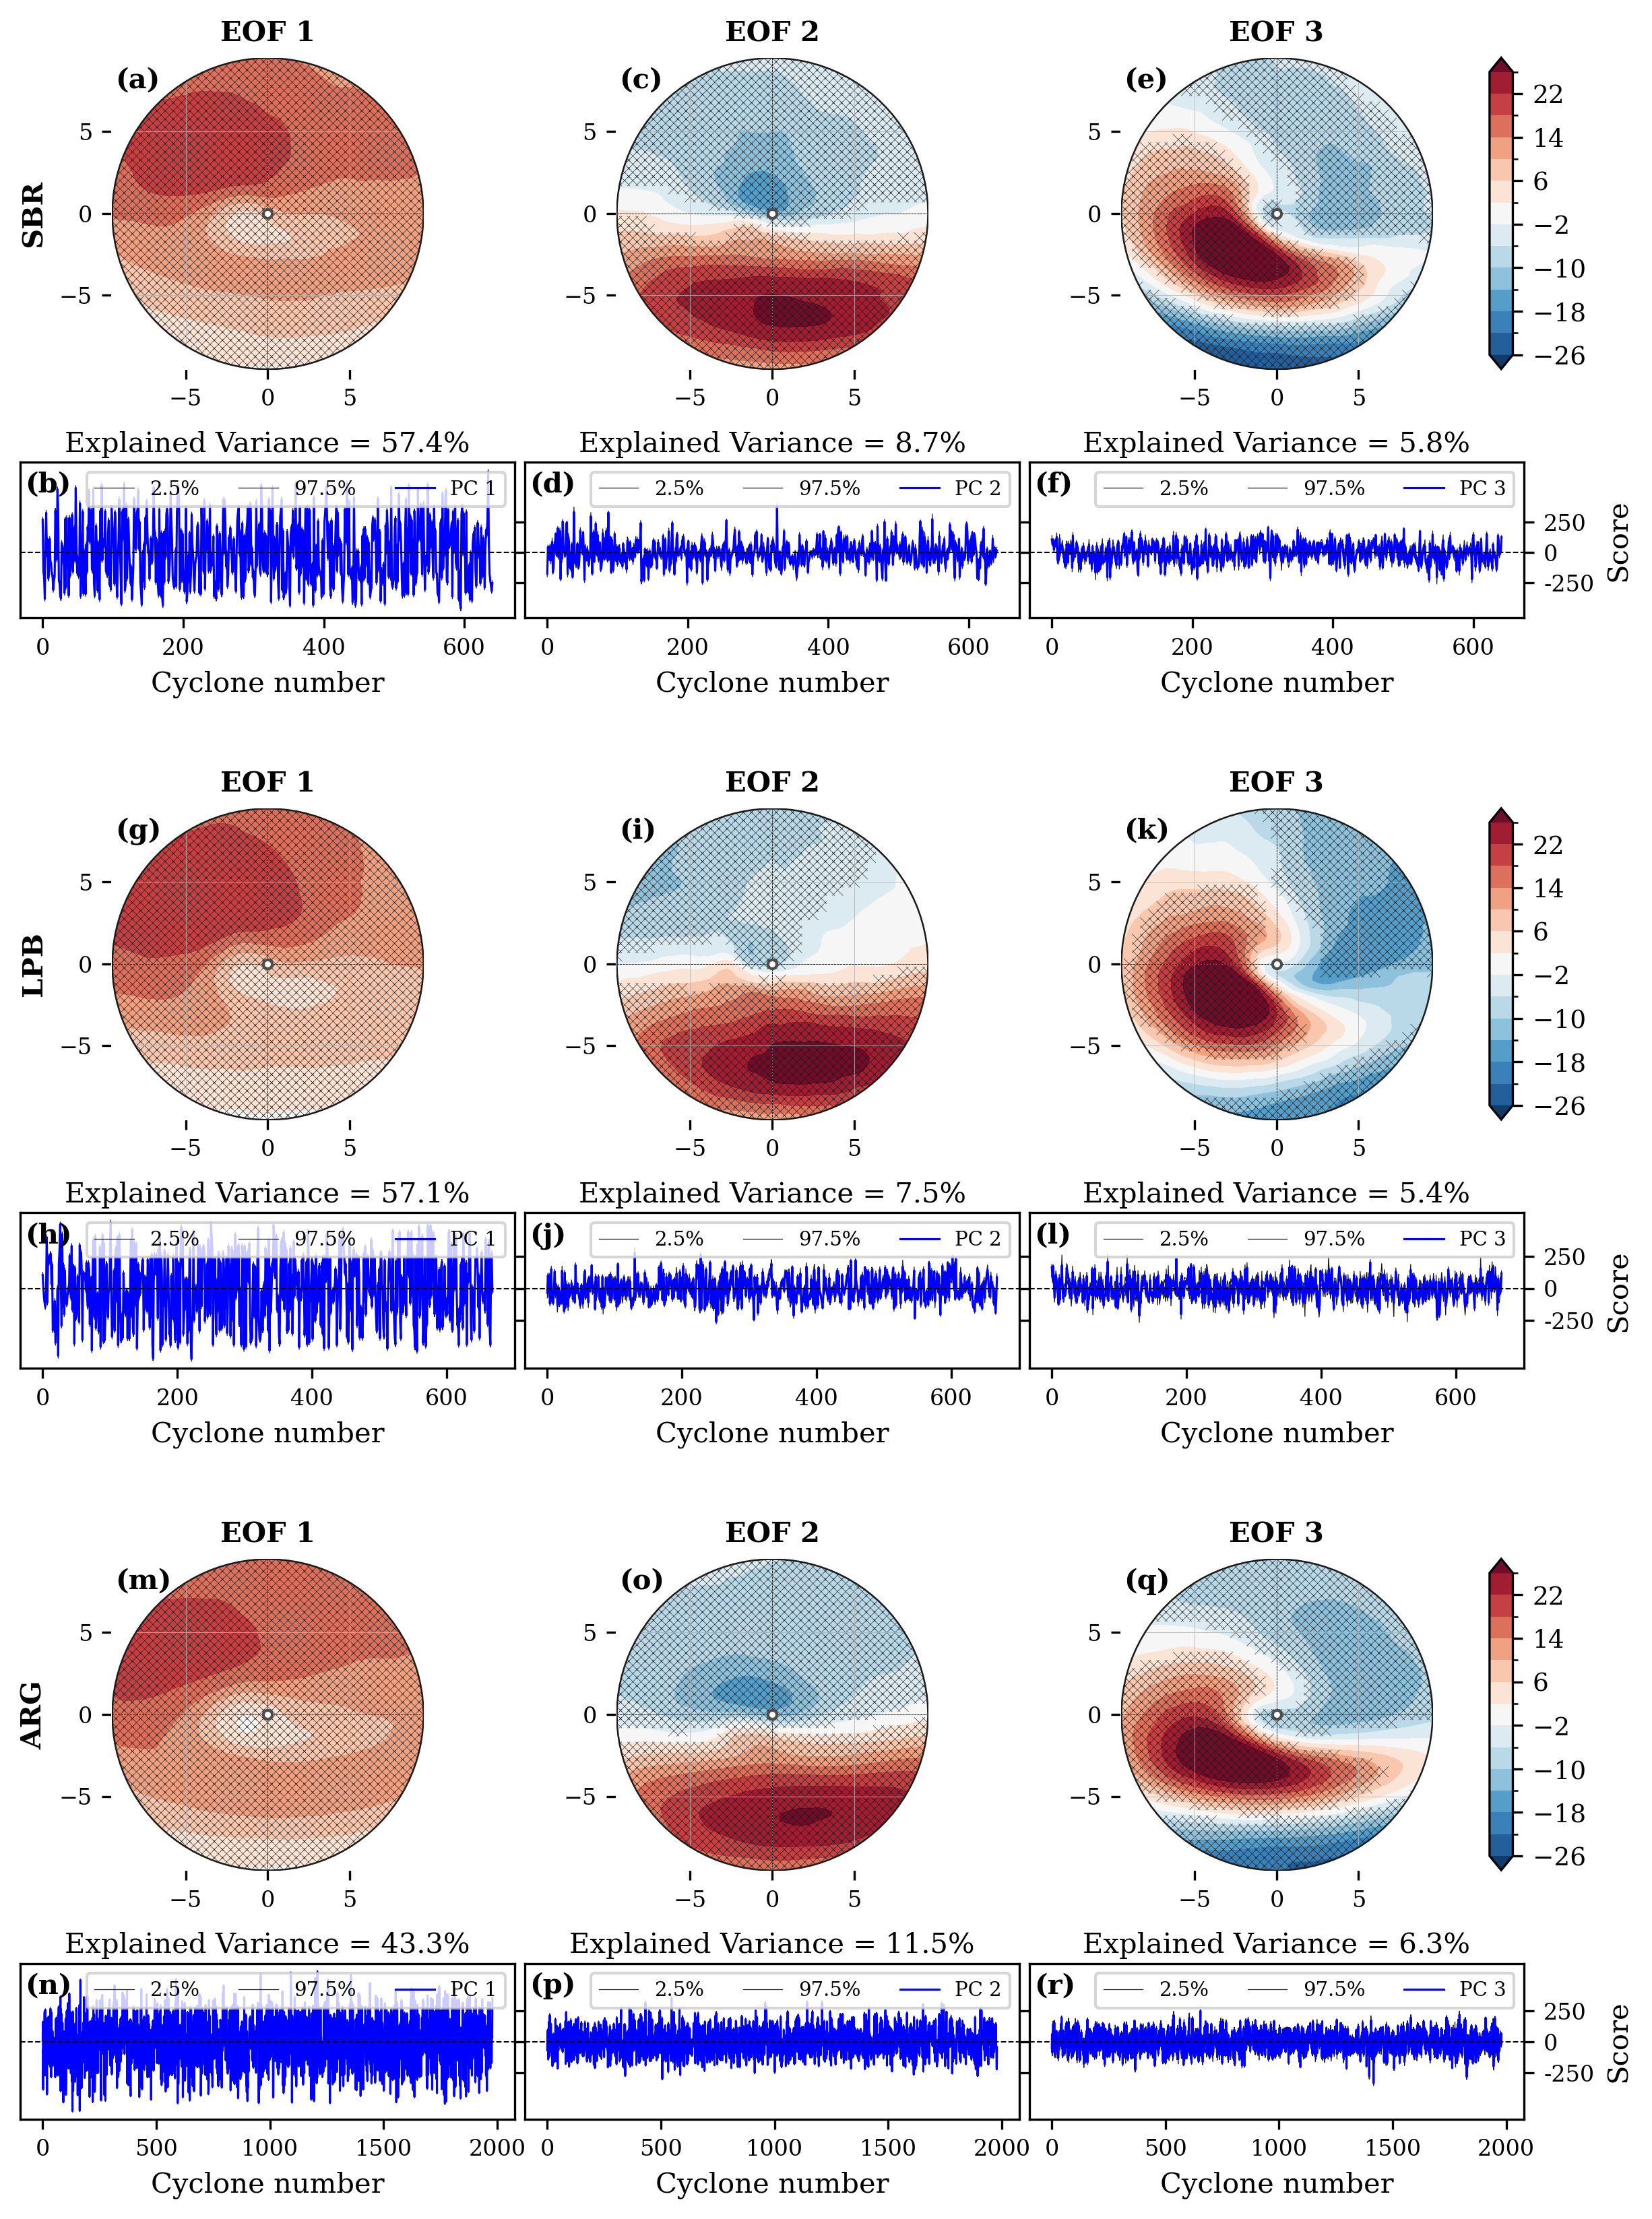
\includegraphics[width=\textwidth]{images/w10/xeof_global_wind10_mature.png}
\caption[Significância espacial dos EOFs em fase de maturidade (População Global)]{Decomposição EOF do vento a 10~m para a População Global em fase de maturidade. Painéis (a, g, m): mapas de EOF1 para SBR, LPB e ARG respectivamente; (c, i, o): EOF2; (e, k, q): EOF3. O hachurado indica significância estatística a 95\% (teste Bootstrap-t; Seção~\ref{subsec:bootstrap_significancia}). Painéis (b, h, n): componentes principais PC1; (d, j, p): PC2; (f, l, r): PC3. A linha cinza delimita os percentis 2.5 e 97.5 da distribuição bootstrap.}
\label{fig:xeof_madurez_global}
\end{figure}

\begin{figure}[htbp]
\centering
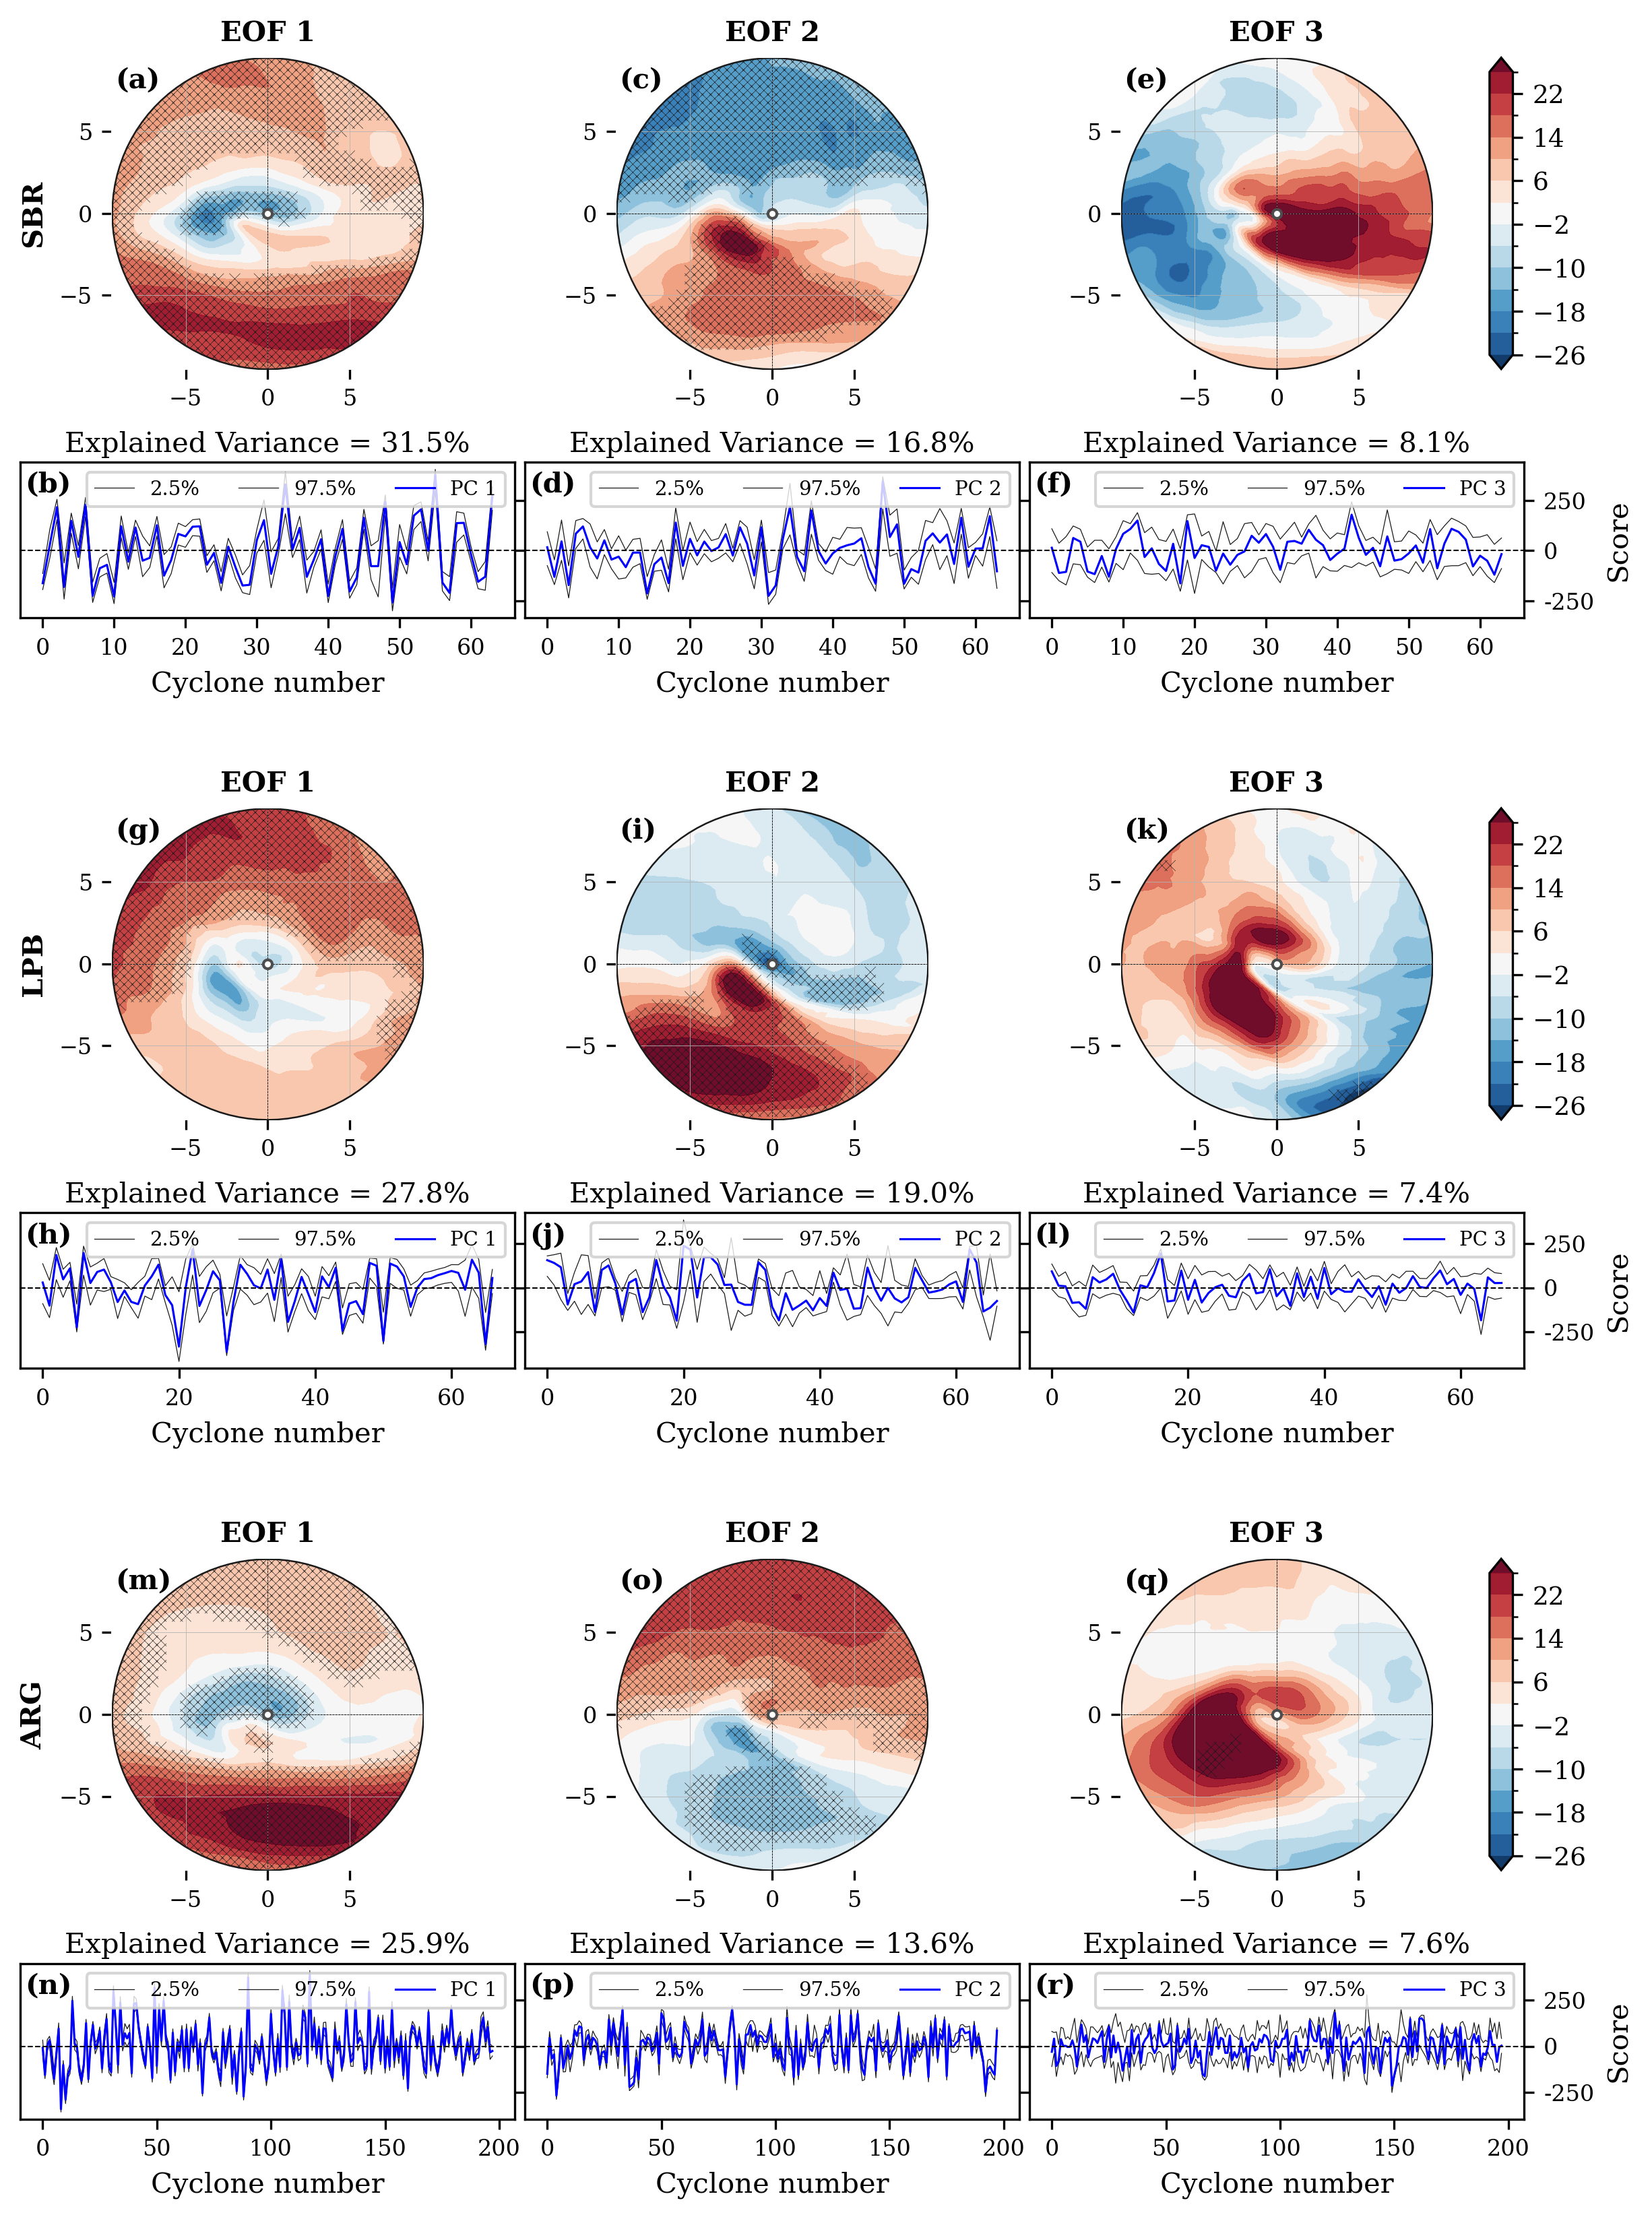
\includegraphics[width=\textwidth]{images/w10/xeof_p90_wind10_mature.png}
\caption[Significância espacial dos EOFs em fase de maturidade (subconjunto p90)]{Decomposição EOF do vento a 10~m para o subconjunto intenso (p90) em fase de maturidade. A disposição de painéis é idêntica à Figura~\ref{fig:xeof_madurez_global}.}
\label{fig:xeof_madurez_p90}
\end{figure}

Na População Global (Figura~\ref{fig:xeof_madurez_global}), EOF1 é significativo em todo o domínio nas três regiões (painéis a, g e~m).
Em concordância com sua alta variância explicada (43--57\%), as componentes PC1 (painéis b, h e~n) apresentam amplitudes maiores do que as de PC2 e PC3 nas três regiões.

EOF2 e EOF3 são significativos na maior parte de sua estrutura, e só perdem significância na transição entre seus polos, onde os valores são próximos de zero. EOF2 mostra um dipolo norte--sul nas três regiões, com valores negativos ao norte e positivos ao sul (painéis c, i e~o), e EOF3 um dipolo nordeste--sudoeste em SBR (painel~e) e leste-nordeste--oeste-sudoeste em LPB e ARG (painéis k e~q). Por construção, EOF2 representa a variância ortogonal ao modo dominante \citep{hannachi2007empirical}, e nesse campo de vento descreve uma oscilação norte--sul que abrange todo o domínio, diferentemente das estruturas compactas próximas do núcleo que o EOF2 de p90 apresenta.

As componentes PC2 e PC3 apresentam amplitudes semelhantes entre si e menores do que as de PC1 nas três regiões (painéis d, f, j, l, p e~r), em concordância com sua menor variância explicada (EOF2: 7.5--11.5\%, EOF3: 5.4--6.3\%). Como na População Global a separação entre autovalores é grande, os modos secundários descrevem uma variabilidade residual. Ainda assim, EOF2 explica mais variância em ARG (11.5\%) do que em SBR (8.7\%) e LPB (7.5\%), o que sugere processos mais complexos em ARG durante a maturidade. Já o EOF3 explica uma variância semelhante nas três regiões e tem uma estrutura parecida, o que indica que esse dipolo é uma fonte comum de variabilidade residual na maturidade.

Em p90 (Figura~\ref{fig:xeof_madurez_p90}), a significância de EOF1 se limita aos valores altos e médios do padrão e não inclui os valores próximos de zero. Em SBR (painel~a) e ARG (painel~m), tanto as anomalias positivas quanto o núcleo negativo próximo do centro são significativos, enquanto em LPB (painel~g) apenas as anomalias positivas o são, e o núcleo negativo não é significativo. Portanto, em SBR e ARG o EOF1 representa de forma robusta tanto a estrutura de maior escala quanto o núcleo localizado próximo do centro, enquanto em LPB apenas a primeira.

Diferentemente da População Global, onde EOF2 e EOF3 descrevem uma variabilidade residual, em p90 EOF2 (painéis c, i e~o) é significativo em ambos os sinais nas três regiões, exceto nos valores próximos de zero, com uma extensão comparável à de EOF1. EOF3 (painéis e, k e~q), por sua vez, praticamente não apresenta áreas significativas. EOF2 mostra estruturas compactas próximas do núcleo nas três regiões, na zona onde costuma se localizar o jato do CCB, na cauda da frente curvada (\textit{bent-back front}), onde \citet{schemm2014linkage} situam os ventos mais intensos em níveis baixos (Seção~\ref{subsec:tb_modelos}).

As componentes principais mostram o mesmo. Em p90, as amplitudes de PC2 (painéis d, j e~p) são semelhantes às de PC1 (painéis b, h e~n), enquanto as de PC3 (painéis f, l e~r) são claramente menores. Diferentemente da População Global, onde PC2 e PC3 têm amplitudes semelhantes entre si e menores do que PC1, em p90 apenas PC2 se aproxima do modo dominante, em concordância com o achatamento do espectro de autovalores (Seção~\ref{sec:var_exp_wind10}) e com o fato de que o EOF3 quase não apresenta áreas significativas.

Em conjunto, na População Global o EOF1, significativo em todo o domínio, permite descrever o campo de vento com um único modo dominante. Em p90, por sua vez, o EOF2 também é significativo e representa parte da variabilidade próxima do núcleo, onde se concentram os ventos mais intensos, o que indica que esse padrão é recorrente entre os ciclones intensos, além do mecanismo físico que se lhe atribua.

\section{Componentes principais (PC1--PC3)}\label{subsec:res_dinamica_pc1}

A distribuição da variância entre vários modos em p90 (Seção~\ref{sec:var_exp_wind10}) se reflete também nas componentes principais. Na População Global, PC1 apresenta amplitudes maiores do que as de PC2 e PC3, enquanto em p90 as amplitudes de PC2 se aproximam das de PC1 (Figura~\ref{fig:xeof_madurez_p90}). Embora PC1 mantenha uma correlação significativa com a vorticidade em todas as fases, em p90 PC2 e PC3 também apresentam correlações de magnitude comparável (Seção~\ref{subsec:pc1_p90_wind10}).

\begin{table}[htbp]
\centering
\caption[Momentos estatísticos e correlação de PC1--PC3 do vento a 10 m - População Global]
{Assimetria ($\gamma_1$) e curtose ($\gamma_2$) da PC1 do vento a 10 metros, e correlação de Spearman em valor absoluto ($|r|$) entre PC1, PC2 e PC3 e a vorticidade relativa a 850 hPa associada à fase, para a População Global. Reporta-se o valor absoluto porque o sinal da correlação depende da convenção de sinal arbitrária de cada EOF (Seção~\ref{subsec:analisis_pc}); o relevante é a magnitude da correlação e sua significância. Os valores significativos ($p<0.05$) são mostrados em negrito.}
\label{tab:stat_global_w10}
\begin{tabular*}{\textwidth}{@{\extracolsep{\fill}}llrrrrr}
\hline
\textbf{Região} & \textbf{Fase} & \textbf{Assimetria ($\gamma_1$)} & \textbf{Curtose ($\gamma_2$)} & \textbf{$|$PC1$|$} & \textbf{$|$PC2$|$} & \textbf{$|$PC3$|$} \\
\hline
\textbf{SBR} & Incipiente       & 0.58  & -0.12 & \textbf{0.57} & \textbf{0.20} & \textbf{0.37} \\
             & Intensificação & 0.26  & -0.91 & \textbf{0.80} & 0.02 & \textbf{0.32} \\
             & Maturidade         & 0.30  & -0.86 & \textbf{0.89} & 0.04 & \textbf{0.25} \\
             & Decaimento     & 0.24  & -0.79 & \textbf{0.83} & \textbf{0.12} & \textbf{0.13} \\
\hline
\textbf{LPB} & Incipiente       & 0.99  & 1.32  & \textbf{0.35} & \textbf{0.14} & \textbf{0.16} \\
             & Intensificação & 0.17  & -1.03 & \textbf{0.71} & \textbf{0.18} & \textbf{0.12} \\
             & Maturidade         & -0.09 & -1.01 & \textbf{0.87} & \textbf{0.09} & \textbf{0.19} \\
             & Decaimento     & -0.11 & -0.77 & \textbf{0.83} & \textbf{0.11} & \textbf{0.09} \\
\hline
\textbf{ARG} & Incipiente       & 0.31  & -0.13 & \textbf{0.43} & \textbf{0.24} & \textbf{0.06} \\
             & Intensificação & -0.22 & -0.37 & \textbf{0.67} & \textbf{0.11} & \textbf{0.05} \\
             & Maturidade         & -0.12 & -0.43 & \textbf{0.86} & \textbf{0.05} & \textbf{0.26} \\
             & Decaimento     & -0.06 & -0.30 & \textbf{0.76} & 0.04 & \textbf{0.28} \\
\hline
\end{tabular*}
\end{table}


\subsection{Relação com a intensidade na População Global}\label{subsec:pc1_global_wind10}

A Tabela~\ref{tab:stat_global_w10} apresenta a assimetria e a curtose de PC1, e a correlação de Spearman em valor absoluto entre PC1, PC2 e PC3 e a vorticidade relativa a 850~hPa de cada fase, para a População Global (Seção~\ref{subsec:analisis_pc}).

Na intensificação e na maturidade, a curtose de PC1 varia entre $-0.37$ e $-1.03$ nas três regiões, o que indica distribuições platicúrticas, sem caudas extremas. LPB apresenta a distribuição mais assimétrica na fase incipiente (assimetria $+0.99$, curtose $+1.32$), enquanto SBR e ARG são mais homogêneas desde as primeiras fases. A correlação de PC1 com a vorticidade aumenta em magnitude em todas as regiões desde a fase incipiente, entre $|r|=0.35$ (LPB) e $0.57$ (SBR), até um máximo na maturidade ($|r|=0.89$ em SBR, $0.87$ em LPB e $0.86$ em ARG), e diminui levemente no decaimento ($|r| > 0.75$). Isso indica que a posição de cada ciclone em relação ao padrão dominante está cada vez mais associada à sua intensidade à medida que o vórtice matura. PC2 é significativa na maioria das combinações de região e fase, com magnitudes fracas ($|r| \leq 0.24$), enquanto PC3 é significativa nas doze combinações e alcança $|r|=0.37$ (SBR incipiente) e $0.32$ (SBR intensificação), valores menores do que os de PC1. Portanto, já na População Global PC2 e PC3 não são puro ruído, embora seu peso seja sempre menor do que o de PC1.
A assimetria de PC1 tende a zero à medida que o vórtice se intensifica, o que indica que os campos de vento se organizam cada vez mais em torno do primeiro modo. Na maioria dos ciclones, o vento se organiza em torno de um padrão coerente (EOF1), enquanto em p90 esse padrão perde dominância sem desaparecer (Seção~\ref{subsec:pc1_p90_wind10}).
SBR apresenta uma correlação moderada desde a fase incipiente, enquanto em LPB a correlação aumenta de forma marcada na intensificação ($|r|$ de $0.35$ para $0.59$). Essa mudança poderia estar relacionada ao estabelecimento do forçante baroclínico nessa fase (Seção~\ref{subsec:tb_lpb}) e coincide com a fase em que a PDFe de LPB alcança sua maior densidade (Seção~\ref{sec:kde_espacial_global}).

\begin{table}[htbp]
\centering
\caption[Momentos estatísticos e correlação de PC1--PC3 do vento a 10 m - Subconjunto p90]
{Assimetria ($\gamma_1$) e curtose ($\gamma_2$) da PC1 do vento a 10 metros, e correlação de Spearman em valor absoluto ($|r|$) entre PC1, PC2 e PC3 e a vorticidade relativa a 850 hPa associada à fase, para o subconjunto extremo (p90). Reporta-se o valor absoluto porque o sinal da correlação depende da convenção de sinal arbitrária de cada EOF (Seção~\ref{subsec:analisis_pc}); o relevante é a magnitude da correlação e sua significância. Os valores significativos ($p<0.05$) são mostrados em negrito.}
\label{tab:stat_p90_w10}
\begin{tabular*}{\textwidth}{@{\extracolsep{\fill}}llrrrrr}
\hline
\textbf{Região} & \textbf{Fase} & \textbf{Assimetria ($\gamma_1$)} & \textbf{Curtose ($\gamma_2$)} & \textbf{$|$PC1$|$} & \textbf{$|$PC2$|$} & \textbf{$|$PC3$|$} \\
\hline
\textbf{SBR} & Incipiente       & 0.16  & -0.56 & \textbf{0.53} & 0.08 & \textbf{0.58} \\
             & Intensificação & -0.25 & -0.65 & \textbf{0.45} & \textbf{0.27} & \textbf{0.58} \\
             & Maturidade         & 0.36  & -0.55 & \textbf{0.44} & 0.19 & 0.12 \\
             & Decaimento     & 1.15  & 3.95  & \textbf{0.66} & \textbf{0.37} & 0.20 \\
\hline
\textbf{LPB} & Incipiente       & 0.77  & 0.42  & \textbf{0.43} & 0.08 & 0.17 \\
             & Intensificação & -0.88 & 0.96  & \textbf{0.45} & \textbf{0.38} & \textbf{0.49} \\
             & Maturidade         & -0.93 & 0.60  & \textbf{0.37} & 0.04 & 0.23 \\
             & Decaimento     & -0.20 & -0.18 & \textbf{0.54} & \textbf{0.37} & \textbf{0.56} \\
\hline
\textbf{ARG} & Incipiente       & 0.29  & -0.14 & \textbf{0.43} & \textbf{0.21} & 0.09 \\
             & Intensificação & -0.38 & -0.19 & \textbf{0.32} & \textbf{0.15} & \textbf{0.38} \\
             & Maturidade         & 0.41  & 0.25  & \textbf{0.26} & \textbf{0.32} & \textbf{0.33} \\
             & Decaimento     & 0.51  & 1.66  & \textbf{0.74} & 0.04 & \textbf{0.20} \\
\hline
\end{tabular*}
\end{table}


\subsection{Relação com a intensidade no subconjunto p90}\label{subsec:pc1_p90_wind10}

A Tabela~\ref{tab:stat_p90_w10} apresenta as mesmas estatísticas para p90. Diferentemente da precipitação (Seção~\ref{subsec:pc1_p90_tp}), a correlação entre PC1 e a vorticidade se mantém significativa em p90 nas três regiões e nas quatro fases, embora com valores de menor magnitude do que na População Global, entre $|r|=0.26$ (ARG, maturidade) e $0.74$ (ARG, decaimento). Isso indica que, mesmo nos ciclones mais intensos, a organização do vento em torno do modo dominante continua associada à intensidade do sistema.

Na intensificação, LPB apresenta uma distribuição leptocúrtica ($\gamma_2 = +0.96$) com assimetria negativa ($\gamma_1 = -0.88$), ou seja, com um pico agudo e alguns casos atípicos em direção a valores baixos. SBR mantém distribuições estáveis durante o desenvolvimento, mas no decaimento apresenta uma curtose muito alta ($\gamma_2 = +3.95$) e assimetria positiva ($+1.15$), o que sugere que os ciclones intensos não seguem um único caminho até a dissipação.

O traço distintivo de p90 não é a perda de correlação de PC1 com a vorticidade, mas sim que PC2 e PC3 apresentam correlações de maior magnitude do que na População Global (Seção~\ref{subsec:pc1_global_wind10}), embora significativas em menos combinações. PC3 supera até mesmo PC1 em SBR durante a fase incipiente ($|r|=0.58$ contra $0.53$) e a intensificação ($0.58$ contra $0.45$), e em LPB durante a intensificação ($0.49$ contra $0.45$) e o decaimento ($0.56$ contra $0.54$). Em ARG, PC2 e PC3 são significativas junto com PC1 durante a maturidade ($|r|=0.32$ e $0.33$, respectivamente), e no decaimento apenas PC3 ($|r|=0.20$). Isso concorda com a distribuição da variância entre vários modos em p90 (Seção~\ref{sec:var_exp_wind10}) e indica que os modos secundários também estão associados à intensidade do vórtice.

Consequentemente, nos ciclones mais intensos a PC1 não resume por si só a organização do vento, já que os modos secundários, que poderiam representar estruturas de mesoescala, também estão associados à intensidade, e descrever o vento desses ciclones apenas com o modo dominante resultaria incompleto. Essa limitação se relaciona com o apontado por \citet{sinclair1997objective}, que mostra que a circulação, ao integrar o tamanho e a rotação do sistema, é uma medida mais representativa da intensidade de um ciclone do que a vorticidade local.

\section{Síntese}\label{sec:sintesis_wind10}

A análise do vento a 10~m mostra que os ciclones intensos não são uma versão amplificada da população média, mas diferem na magnitude, na localização e na organização espacial de seus ventos máximos.

\paragraph{Magnitude.}
Na População Global, a moda dos máximos de vento se situa entre 11 e 14~m\,s$^{-1}$ na fase incipiente e entre 16 e 19~m\,s$^{-1}$ na maturidade. Em p90, a moda da maturidade se desloca para 23--25~m\,s$^{-1}$, entre 25\% e 50\% acima da População Global, com caudas de até 30~m\,s$^{-1}$, valores coerentes com os reportados para ciclones do Atlântico Sul. Os picos de p90 são semelhantes entre regiões, embora ARG estenda mais sua cauda em direção a velocidades altas.

\paragraph{Localização.}
Na População Global, os máximos se distribuem de forma difusa e se deslocam do setor leste nas primeiras fases ao quadrante noroeste na maturidade. Em p90, esse deslocamento é mais marcado, e na maturidade os máximos se concentram fortemente no quadrante noroeste, a ${\sim}$2--4$^{\circ}$ do centro, na zona onde a literatura situa o jato da cinta transportadora fria (CCB) e a fratura frontal. Essa concentração é maior em SBR e LPB do que em ARG, embora SBR apresente a distribuição de magnitudes mais larga das três regiões, o que indica que concentrar a localização dos máximos não implica concentrar sua magnitude. No decaimento, o núcleo de p90 permanece no noroeste, enquanto na População Global a densidade diminui e sua localização varia entre regiões.

\paragraph{Padrões de variabilidade.}
Na População Global, EOF1 explica entre 30.9\% e 57.4\% da variância, forma um gradiente norte--sul de grande escala e é significativo em todo o domínio, de modo que um único modo descreve grande parte da variabilidade do vento. Em p90, EOF1 não supera 37.6\% e a variância se distribui entre vários modos. Na maturidade, EOF1 apresenta um núcleo negativo compacto próximo do centro, significativo em SBR e ARG mas não em LPB, e EOF2 é significativo com uma extensão comparável à de EOF1 e estruturas compactas próximas do núcleo, enquanto EOF3 quase não apresenta áreas significativas. Essa organização é compatível com um maior peso da variabilidade de mesoescala nos ciclones intensos.

\paragraph{Relação com a intensidade.}
Na População Global, a correlação entre PC1 e a vorticidade aumenta até valores de $|r|=0.86$ a $0.89$ na maturidade. Em p90, mantém-se significativa em todas as regiões e fases, embora com valores de menor magnitude (entre $|r|=0.26$ e $0.74$), diferentemente do que ocorre com a precipitação (Capítulo~\ref{cap:resultados_tp}). Ao mesmo tempo, PC2 e PC3 apresentam em p90 correlações de maior magnitude do que na População Global, e em quatro combinações de região e fase superam as de PC1. Nos ciclones intensos, o modo dominante não resume por si só a relação entre a organização do vento e a intensidade do sistema.

\paragraph{Alcance.}
Esses resultados dependem da vorticidade de cada fase como medida pontual de intensidade e poderiam diferir com uma medida integrada de circulação \citep{sinclair1997objective}. Além disso, o ERA5 tende a subestimar as magnitudes extremas (Seção~\ref{sec:datos_era5}), e a relação do núcleo noroeste com o \textit{sting jet} e o CCB se apoia principalmente em estudos do Hemisfério Norte e na simetria entre hemisférios, já que a climatologia global desses sistemas não distingue o Atlântico Sul \citep{gray2024global}.

O Capítulo~\ref{cap:resultados_tp} aplica a mesma análise à precipitação, e o Capítulo~\ref{chap:meof} avalia se os máximos de ambas as variáveis coincidem no espaço segundo a fase e a região de gênese (Seção~\ref{sec:tb_compound_def}).
